%%%%%%%%%%%%%%%%%%%%%%%%%%
\chapter{MATERIALS AND METHODS} \label{chap:3}
%%%%%%%%%%%%%%%%%%%%%%%%%%
\def\etal{{\it et al.}\/}
%%%%%%%%%%%%%%%%%%%%%%%%%%
\section{Introduction}
%%%%%%%%%%%%%%%%%%%%%%%%%%
\begin{sloppypar}
Materials are mainly found in three phases; solids, liquids and gases. Most of the molecular/atomic properties of materials are based on their existing phase. In gaseous phase, the molecules are at long distance and arranged in random manner. Thus the material density and intermolecular interaction is low at the normal temperature and pressure~\citep{Frenkel2002}. The molecules in liquid phase have only short-range arrangement 
and density is larger than that in gaseous phase. The interatomic/molecular interactions in liquids is stronger than to those in gaseous phases, respectively. In solids, the atoms or/and molecules have long-range arrangement with the highest atomic packing. This causes the highest density and the strongest interaction in between the constituent particles. Based on these properties, it is understood that the arrangement of the particles and nature of their interaction differ from one phase to another~\citep{Hansen2006}.  In this context, one can consider the atomistic level of study to understand the microscopic properties of a material where the separate identity of electrons is neglected. For nanostructures, however, diagnosis of electronic properties is essential to understand their basic physics and chemistry. Hence the basic techniques to study their properties differ on the basis of their atomic/molecular arrangement and properties of interest.
\end{sloppypar}

In the present work, we study the structural and transport and thermodynamic properties of  nitric oxide NO, CO, N2, alkali-halide ions in water  using empirical potential from molecular dynamics simulation technique at different temperatures. Then, We discuss the transport and thermodynamic properties of light alkanes (methane, ethane, propane and n-butane) in water. In addition, we perform  the atomistic level of calculations by incorporating empirical force field for the study of free energy of solvation of light alkanes in different liquid media (water and  methanol). In this chapter, we begin our discussion from the theoretical background and then move into the systems considered for the present work. 

\begin{enumerate}[(a)]
\item Many physically-based numerical simulations model easily observable real world phenomena.
\item Molecular Dynamics (MD) simulations model things that are too small for us to observe directly.
\item Modeling the motion of a complex molecular problems and solving the problems by  the 
wave-function and density-functional theory methods of calculations would be accurate. But it would also be very difficult to program and take more computing power than anyone has.  Therefore, we can not use quantum mechanical methods to solve the larger or complex systems. 
\item Instead of using Quantum Mechanics, we can use classical Newtonian mechanics to model our system.
This is a simplification of what is actually going on, and is therefore less accurate. To alleviate this problem, we use numbers derived from quantum mechanical calculations or ab-initio calculations for the constants in our classical equations.
\item  Molecular dynamics (MD) is  numerical method for studying many-particle systems such as molecules, clusters, and even macroscopic systems such as gases, liquids and solids. It is 
used extensively in materials sciences, chemical physics, and biophysical-chemistry.
\end{enumerate}

%%%%%%%%%%%%%%%%%%%%%%%%%%
\section{Statistical Mechanics and  Ensembles}
%%%%%%%%%%%%%%%%%%%%%%%%%%
Statistical Physics is the study of the special laws which govern the behavior and properties of macroscopic systems (that is, systems formed of a very large number of individual particles, such as atoms and molecules). To a substantial limit the general character of these laws does not depend on the mechanics (classical or quantum) which describes the motion of the individual particles in a body, but their confirmation asks a different argument in the two cases. In principle, we can obtain complete information concerning the motion of a mechanical system by constructing and integrating the equations of motion of the system, which are equal in number to its degrees of freedom. On the other hand,  if we consider a system which has a very large number of degrees of freedom, the actual application of the methods of mechanics demands the setting up and solving the same number of differential equations, which in general is not applicable. It should be stressed that it would be completely impossible to substitute in the general solution the initial conditions for the velocities and coordinates of all the particles, even if we could integrate these equations in a general form. That means, we can conclude that as the number of particles increases, the complexity and intricacy of the properties of the mechanical system increases, and  no trace of regularity can be found in the behavior of a macroscopic system. Thus, even though the motion of systems with a very large number of degrees of freedom obeys the same laws of mechanics as that of systems consisting of a small number of particles, the existence of many degrees of freedom results in laws of a different kind. The importance of statistical physics in many other branches of theoretical  physics is due to the fact that in Nature we continually encounter macroscopic bodies whose behavior can not be fully described by the methods of mechanics alone, for the reasons mentioned above, and which obey statistical laws ~\citep{Landau1980}.

In Statistical Physics, system under consideration can be studied with few macroscopic properties such as temperature (T), pressure (P) and volume (V). If these three quantities have uniform value we can state that we have one macroscopic realization of a system. On the other hand, this state can be achieved through numerous microscopic realizations of the system. Molecules in a system can have for example same average velocity in many different ways. Gibbs introduced the idea of a statistical ensemble to describe a macroscopic system.
A state of a system under consideration can be specified by the 3N canonical
coordinates $q_1,..., q_{3N}$ and their conjugate momenta $p_1,..., p_{3N}$. The 6N-dimensional space spanned by ${\{q_i, p_i} \}$ is called the $\Gamma$-space, or phase space, of the system. A point in $\Gamma$-space  represents a state of the entire N-particle system, and is referred to as the representative point. Over the time system will pass through multiple points and it will draw a trajectory in phase space. This trajectory is something we could be able to calculate if only we had capabilities to solve $\vec{F} =m\vec{a} $ with adequate initial conditions for all particles under consideration. After long period of time, system will visit every point in phase space although some of the points will be less accessible. To deal with all this we use ensembles. Their description that we like best is maybe the one given by Gibbs who states that ``ensemble is a collection of systems, identical in composition and macroscopic condition but existing in different states''. According to Gibbs, an ensemble is geometrically represented by a distribution of representative points in $\Gamma$-space, usually a continuous distribution, a density function $\rho$(p, q, t). The density function $\rho(p, q, t)$,  is so defined that $\rho(p, q, t)$ $d^{3N}p~d^{3N}q$, is the number of representative points that at time $t$ are contained in the infinitesimal volume element $d^{3N}p~d^{3N}q$ of $\Gamma$-space centered about the point $(p, q)$, with  $(p, q)$ is an abbreviation for ($p_1$,..., $p_{3N}$; $q_1$,..., $q_{3N}$). It is to be emphasized that members of an ensemble are mental copies of a system and do not interact with one another ~\citep{huang2009}.
 
Given $\rho (p, q, t)$ at any time $t$, its subsequent values are determined by the dynamics of molecular motion. Let the Hamiltonian of a system in the ensemble be ${H}$($p_1$,..., $p_{3N}$; $q_1$,..., $q_{3N}$. The equations of motion for a system are given
by
\begin{eqnarray}\label{hamiltonian}
\dot{p_i} = -\frac{\partial {H}} {\partial q_i}~~~ (i = 1, 2  ...., 3N)\nonumber\\
\dot{q_i} = \frac{\partial {H}} {\partial q_i}~~~ (i = 1, 2  ...., 3N) 
\end{eqnarray}
Eq.(\ref{hamiltonian}) describes us   how a representative point moves in $\Gamma-space$ as time evolves. When we assume that the Hamiltonian does not depend on any time derivative of $p$ and $q$, the Eq. (\ref{hamiltonian} is invariant under time reversal and uniquely determines the motion of a representative point for all times, when the position of the representative point is given at any time. It follows immediately from these observations that the locus of a representative point is either a simple
closed curve or a curve that never intersects itself. Furthermore, the loci of two distinct representative points never intersect ~\citep{huang2009}.

The aim of statistical mechanics is to derive all the equilibrium properties of
a macroscopic molecular system from the laws of molecular dynamics. Thus it
aims to derive not only the general laws of thermodynamics but also the specific
thermodynamic functions of a given system. Classical statistical mechanics is founded on the following postulate.

\begin{enumerate}
\item \textbf{Postulate of Equal a Priori Probability} ~~~~~  When a macroscopic system is in
thermodynamic equilibrium,  its state is  equally likely to be any state satisfying the macroscopic conditions of the system.
\item \textbf{Ergodicity } ~~~~~~ The ensemble average  of a measurable property of the system, such as energy or momentum, say $f(p,q)$ in thermodynamic system of interest is equal to the time average  of $f(p,q)$ taken over a long time interval.
\end{enumerate}
The ensemble average of $f(p, q)$ is defined by
\begin{equation}
\left\langle f \right\rangle_{ensemble} = \frac{\int d^{3N}p~ d^{3N}q~ f(p, q)~ \rho (p,q)} {\int d^{3N}p~ d^{3N}q~ \rho (p,q)}
\end{equation}
The time average of  $f(p, q)$ is defined by 
\begin{equation}
\left\langle f \right\rangle_{time} = \lim_{t\to\infty} \frac{1}{t} \int_{0}^{t} f(p, q) ~ dt
\end{equation}
In MD simulations, solving the physical problems on a computer, for large number of particles, the experimentally observable macroscopic property $f_{obs}$ can be written as \citep{huang2009, Allen1989}
\begin{equation}
 f _{obs} = \left\langle f \right\rangle_{ensemble} = \left\langle f \right\rangle_{time}
\end{equation}
Time average and ensemble average are usually taken as the same thing but that  doesn't need to always be true. If a system has this property it's said to be ergodic, and equivalence of time and ensemble averages itself is called ergodicity. Ensemble is then assembly of all possible micro-states that can be achieved by a system under imposed macroscopic conditions. Ensembles can be divided according to macroscopic quantities that hold constant value. Some of the common  types of ensembles are:
\begin{itemize}
\item Microcanonical ensemble (N, V, E)
\item Canonical ensemble (N, V, T)
\item Grand canonical ensemble ($\mu$, V, T)
\item  Isothermal-isobasic - ensemble (N, P, T)
\item Isoenthalpic-isobaric -  ensemble (N, P, H)
\end{itemize}

\begin{figure}[h!]
\centering
\includegraphics[width=15.5cm,height=5.5cm]{Chapter3/Statistical_Ensembles.png}
\caption[Visual representation of different statistical ensembles.]{Visual representation of different statistical ensembles. (\url{https://en.wikipedia.org/wiki/Statistical Ensemble/(mathematical physics)} dated: May 5, 2018.)}
\end{figure}

%%%%%%%%%%%%%%%%%%%%%%%%%%
\subsection{Microcanonical Ensemble} 
%%%%%%%%%%%%%%%%%%%%%%%%%%
This ensemble represents all states that have fixed total energy, number of particles and volume. That means in this ensemble the macrostate of a system is defined by the number of molecules $N$, the volume $V$ and the energy $E$. However, from a practical point of view, an absolutely isolated system is too much of an idealization and its energy cannot be defined sharply.  Therefore, in the microcanonical ensemble every system has $N$ molecules, a volume $V$, and an energy between $E$ and $E + \Delta$, $\Delta \ll  E $. Now, the microcanonical ensemble is a collection of systems for which the density function $\rho $  is given by \citep{huang2009, pathria1996}:
\begin{eqnarray}
\rho (p,q)= \begin{dcases}
    Const. & \text{if }  E \leq H(p,q)\leq  E+ \Delta \\
    0,              & \text{otherwise}
\end{dcases} 
\end{eqnarray}
The fundamental quantity that furnishes the connection between the microcanonical ensemble and thermodynamics is the entropy. It is the main task of this section to define the entropy and to show that it possesses all the properties attributed to it in thermodynamics.\\
Let $\Gamma(E) $  and  $\Sigma (E)$  denote the volume in $\Gamma $ space occupied by the microcanonical ensemble and  the volume in $\Gamma $ space enclosed by the energy surface of energy $E$ respectively: 
\begin{align}
\Gamma(E) &= \int_{E \leq H(p, q)\leq  E+ \Delta} d^{3N}p~ d^{3N}q  \\
\Sigma (E) & = \int_{ H(p, q)\leq  E } d^{3N}p~ d^{3N}q 
\end{align} and then 
\begin{equation}
\Gamma(E) = \Sigma (E + \Delta ) - \Sigma (E) 
\end{equation}
If $\Delta $ is so chosen that $\Delta \ll E $, then
\begin{equation}
\Gamma(E) = \omega (E) ~ \Delta
\end{equation}
where $\omega(E)$ is called the density of states of the system at the energy $E$ and is
defined by 
\begin{equation}
\omega(E)= \frac{\partial \Sigma (E)}{\partial E}
\end{equation}
 The entropy is defined by the following relations which are equivalent to each other 
 \begin{align}
 S &= k_B~log~\Gamma(E) \nonumber \\
 S &= k_B~log~\omega(E) \\
 S &= k_B~log~\Sigma(E) \nonumber
 \end{align}
 where, $k_B$ is is a universal constant,  Boltzmann's constant. \\
 Other thermodynamic quantities, absolute temperature (T),  pressure (P), internal energy (U), Helmholtz free energy (A), Gibbs free energy (G), heat capacity at constant volume ($C_V$), can be obtained from entropy with use of Maxwell thermodynamical  relations \citep{huang2009}: 
 \begin{align}
  U (S, V)& = E (S, V) \nonumber \\
    T & = \left(  \frac{ \partial U} {\partial S }\right)_V  \nonumber \\
   P  &  = - \left(  \frac{ \partial U} {\partial V }\right)_S  \\
    A & = U - T~S \nonumber \\
     G & = A + P~ V = U + P~V - T~ S \nonumber\\
     C_V & = \left(  \frac{ \partial U} {\partial T }\right)_V  \nonumber
 \end{align}
 %%%%%%%%%%%%%%%%%%%%%%%%%%
 \subsection{Canonical Ensemble} 
 %%%%%%%%%%%%%%%%%%%%%%%%%%
 Canonical ensemble represents a system that has constant number of particles, size and temperature. It is an ensemble in which  the macrostate of a system is defined by the number of molecules $N$, the volume $V$ and the temperature energy $T$. A canonical  ensemble is appropriate for the description of a system not in isolation, but in thermal equilibrium with a larger system.  The  canonical ensemble describes those systems which are not isolated but are in thermal contact with the heat reservoir under consideration together with a heat reservoir forms a closed system and then the system of interest is treated as a subsystem of the closed system. For the canonical ensemble,  the density function $\rho $  is given by \citep{huang2009}: 
 \begin{equation}
 \rho (p, q) = e^{-\beta H(p,~ q)} 
 \end{equation} 
 where $\beta = 1/k_B~T$ and $H(p, q)$ is the Hamiltonian of the system. The volume in $\Gamma$ space occupied by the canonical ensemble is called the canonical partition function $Q_N(V, T)$:
 \begin{equation}
 Q_N(V, T) = \frac {1}{N! h^{3N}}\int d^{3N}p~ d^{3N}q ~ e^{-\beta H(p,~ q)}  
 \end{equation} 
 Connection with thermodynamics for this system is Helmholtz free energy $A (V, T)$, which is obtained from the formula: 
 \begin{align}
 Q_N(V,~T) & = e^{-\beta~A(V,~T)}\nonumber\\
 or, ~~ A(V,~T) &= k_B~T~log~Q_N(V,~T)
 \end{align}
 All other thermodynamic functions may be found from $A(V, T)$ by the Maxwell relations in thermodynamics:
 \begin{align}
    S & = -\left(  \frac{ \partial A} {\partial T }\right)_V  \nonumber \\
    P  &  = - \left(  \frac{ \partial A} {\partial V }\right)_T \nonumber \\
    G & = A + P~ V \\
    U &= \left\langle  H \right\rangle  = - \frac{\partial} {\partial \beta } log Q_N(V,~T) = A + T~S \nonumber \\
    \mu & = \left(  \frac{ \partial A} {\partial N }\right)_V \nonumber
  \end{align}
  %%%%%%%%%%%%%%%%%%%%%%%%%%
 \subsection{Isothermal-Isobaric  Ensemble} 
 %%%%%%%%%%%%%%%%%%%%%%%%%%
 This ensemble depicts systems with constant pressure, temperature and number of particles. It is an ensemble in which  the macrostate of a system is defined by the number of molecules $N$, the pressure $P$ and the temperature energy $T$. It is of great importance since these conditions are valid for a large number of systems and it is widely used. We can picture it as a small system inside a big reservoir that keeps its pressure and temperature constant. Constant pressure means that the volume of a system is changing through time. For the isothermal-isobaric ensemble, the density function $\rho $ is given by \citep{Allen1989}: 
 \begin{equation}
 \rho (p, q) = e^{-\beta(H + P~V)} 
 \end{equation} 
 where $\beta = 1/k_B~T$ and $H(p, q)$ is the Hamiltonian of the system. The isobaric-isothermal   partition function $Q_{NPT}$:
 \begin{equation}
 Q_{NPT} = \frac {1}{N! h^{3N}} \int d^{3N}p~ d^{3N}q ~dV ~ e^{-\beta(H + P~V)}  
 \end{equation} 
 Connection with thermodynamics for this system is Gibbs free energy $G$, which is obtained from the formula: 
 \begin{align}
 G & = - k_B~T~log~Q_{NPT} = A + P~V
 \end{align} 
 
 %%%%%%%%%%%%%%%%%%%%%%%%%%
 \section{Structural, Transport and Thermodynamic Properties}
 %%%%%%%%%%%%%%%%%%%%%%%%%%
  A system is not in equilibrium when the distribution function is different from the Maxwell-Boltzmann distribution. The most common case of a nonequilibrium situation is that in which the temperature, density, and average velocity are not constant throughout the system. To approach equilibrium, these nonuniformities have to be resolved through the transport of energy, mass, and momentum
 from one part of the system to another. In MD simulations, we wish to measure interesting properties of many-body systems that can be compared with real experiments. Those properties   include structural, transport, and  thermodynamic properties. The structural properties of the fluid mixture is analyzed by using radial distribution function (RDF). The transport properties includes the physical properties such as  diffusion coefficients, shear viscosity, thermal conductivity, mobility, friction coefficients. The thermodynamic properties of the system under consideration includes the thermodynamical physical quantities such as Temperature $T$, the pressure $P$, the specific heat capacity $C_V$, Gibbs free energy $G$, Helmholtz free energy $A$. The thermodynamic properties also includes free energy of solvation, chemical potential $\mu$ ~\citep{huang2009, Frenkel2002}. In the following section, we  discuss the radial distribution function (RDF), phenomenon of diffusion and diffusion coefficients, free energy of solvation and method of calculations.
 %%%%%%%%%%%%%%%%%%%%%%%%%%
 \subsection{Radial Distribution Function (RDF)}
 %%%%%%%%%%%%%%%%%%%%%%%%%%
  The relative arrangements of atoms and molecules in fluid and solid phases are most often accurately described in terms of the principles of classical statistical mechanics. There are, of course, electrons surrounding the nuclei in these systems, and the behavior of electrons is surely quantum mechanical in nature. Yet after averaging over these quantal fluctuations, the remaining problem is to sample the statistical configurations of the nuclei in the effective interactions induced by the electrons we have already integrated out~ \citep{chandler1987}.
  
 Molecular structure refers to the patterns and correlations that molecules display in
 their placement in space. Molecules are in constant motion, rotating and moving about in erratic ways, so the notion of structure has meaning only in average sense. There
 are many ways to quantify this average structure, one of them is estimation  of radial distribution function. The structure of a simple fluid is characterized by a set of distribution functions for the atomic positions, the simplest of which is the pair distribution function $g(\mathbf{r})$. This function gives the probability of finding a pair of atoms at distance $r$ apart, relative to the probability expected from a completely random distribution at the same density. The pair distribution function $g(\mathbf{r})$ is most simply thought of as the  number of atoms at distance r from a given atom compared with the number at the same distance in an ideal gas at the same density. For an isotropic system, the pair distribution function is a function of only the separation of atoms $r = \lvert\mathbf{r}\rvert $, and is completely defined by the radial distribution function (RDF), denoted by $g(\mathbf{r})$ ~ \citep{Allen1989}. The radial distribution function describes how, on average, the atoms in a system are radially packed around each other.
 
 For a system of fluid of  $N$ particles, volume $V$ and temperature $T$, with density of fluid $\rho = N/V$, the definition of the radial distribution function, g(r),
 infers that $\rho g(r)~d\mathbf{r}$ is the probability of observing  a second molecule in d$\mathbf{r}$  given that there is a molecule at the origin of $\mathbf{r}$. This probability is not normalized to unity, but we have 
 \begin{equation}\label{rdf}
 \int_0^\infty \rho g(r)~4\pi r^2~dr = N-1 \approx N
 \end{equation}
 
 The Eq. (\ref{rdf}) shows that $\rho g(r)~4\pi r^2~dr $   is the number of
 molecule between $r$ and $r + dr$ about a central molecule. When the bulk density $\rho$ is multiplied by the factor $g(r)$, we obtain the  local density $\rho(r) = \rho g(r)$. Since molecules become effectively hard  as $r \longrightarrow 0$, $g \longrightarrow 0$ as $r \longrightarrow 0$. Also, since the influence of molecule at the origin diminishes as r becomes very large, $g \longrightarrow 1$, as $r \longrightarrow \infty$ ~\citep{mcquarrie2000}.
 
 \begin{figure}[h!]
 \centering
 \includegraphics[width=15 cm,height=11 cm]{Chapter3/coordination.png}
 \caption[Simple liquid structure.]{Simple liquid structure~\citep{chandler1987}.}
  \label{coordinationfig} 
 \end{figure}
 
 \begin{figure}[h!]
 \centering
 \includegraphics[width=14 cm,height=11 cm]{Chapter3/rdf.png}
  \caption[The radial distribution function for a simple fluid.]{The radial distribution function for a simple fluid~\citep{chandler1987}.} 
 \label{rdffig} 
 \end{figure}
 
  A schematic view of the liquid structure (drawn in two dimensions for artistic convenience) is shown in Fig. (\ref{coordinationfig}), which shows the most probable location of first and second coordination shell with respect to a fixed molecule. In the figure, $\sigma$ is the van der Waals diameter (which is roughly equal to  the distance of closest approach between two atoms during a physical  encounter), the cross-hatched atom is the reference atom which is at the origin. The atoms are drawn close  together because of typical liquid densities, and  Since the fluid is  dense, there is a strong likelihood that a first neighbor shell will be  found around $r = \sigma$. The nearest neighbors, which comprise the \textit{first  coordination shell}, tend to exclude the next nearest neighbors from an intermediate region around $r = 1.5 \sigma$ and  $g(r)$ will be less than 
  unity in that region, and it will peak above the uncorrelated result 
  near $r = 2\sigma$. The RDF of a liquid and gas phase of argon is shown in Fig. (\ref{rdffig}). For, the  liquid, the second peak corresponds to the most probable
  location for the next nearest neighbors and these neighbors comprise  the \textit{second coordination shell}. This layering manifests the granularity  (non-continuum nature) of the liquid. It shows up in an oscillatory  form for g(r), which persists until r is larger than the range of  correlations (typically a few molecular diameters in a dense liquid). In the dilute gas phase, the range of correlations is just the range of the intermolecular pair potential and there is no layering.   Notice both in the  Fig. (\ref{coordinationfig}) of the liquid  and the Fig. (\ref{rdffig}) of g(r)  that there is a finite density of particles even in ''unlikely'' regions  like $r = 1.5 \sigma $. This is one of the features that distinguishes a liquid from a crystalline solid. Without it, the possibility of diffusion would  be drastically reduced. In crystalline solids, RDF shows sharp peaks and troughs up to infinity where the separations and heights are  the characteristics of the lattice structure. In liquids however, RDF oscillates up to  certain orders and then attains constant value as unity~\citep{chandler1987, mcquarrie2000}.
  
  The radial distribution function or pair distribution function $g_{AB}(r)$ between particles of type $A$ and $B$ is defined in the following way~\citep{Gromacs-manual}: 
  \begin{equation}
  g_{AB}(r) = \frac{\langle \rho_B (r) \rangle}{\langle \rho_B \rangle_{local}} = \frac{1}{\langle \rho_B \rangle_{local}} \frac{1}{N_A}  \sum_{i\in A}^{N_A} \sum_{j\in B}^{N_B} \frac{\delta(r_{ij}-r)}{4\pi r^2}
   \end{equation}
   where $\langle \rho_B (r) \rangle$ is the particle density of type $B$ at a distance $r$ around particles $A$ and  $\langle \rho_B \rangle_{local}$ is the particle density of type $B$ averaged over all the spheres around particles $A$.
   
   The radial distribution function turns out to be of central importance in the theory of liquids for two reasons. First, all the thermodynamic functions can be written in terms of $g(r)$ if we assume the total potential energy of the N-body system is pairwise additive: 
   \begin{equation}
  U_N(r_1, r_2, ..., r_N) = \sum_{i<j} u(r_{ij})
  \end{equation}
  In addition, the radial distribution function can be determined by diffraction studies on liquids. In a solid the molecules are arranged regular repeating order and this leads to a sharp X-ray diffraction pattern from which the order of molecules in solid can be obtained. The X-ray diffraction pattern of liquid is more diffuse but can be used to determine the local short-range order in a fluid as depicted in Fig. (\ref{rdffig}). The peaks in the curve represent the smeared-out shells of first nearest neighbors, second nearest neighbors, etc., which in a sense are remnants of ordering found in the solid ~\citep{chandler1987, mcquarrie2000}. 
  %%%%%%%%%%%%%%%%%%%%%%%%%%
    \subsection{Diffusion and Diffusion Coefficient}
    %%%%%%%%%%%%%%%%%%%%%%%%%%
     There are  different transport phenomenon whereby mass, energy, or momentum are transported from one region of a material to  another under the influence of composition, temperature, or velocity gradient. Diffusion refers to the the movement of matter within a single phase from a region of high concentration to a region of low concentration in the absence of mixing. In diffusion, there
   is a net transfer of diffusing particles from the region of higher concentration to the region of lower concentration as a result of random molecular motions. This definition of diffusion is fundamental throughout science, from gas exchange in the lungs to the spread of carbon dioxide in the atmosphere to the movement of water from one side of a cell's plasma membrane to the other. However, the concept of diffusion is rarely as simple as molecules moving from one place to another. Temperature, the size of the molecules involved, the distance molecules need to travel, the barriers they may encounter along the way, and other factors all influence the rate at which diffusion takes place ~\citep{cussler2009}. 
   
\begin{figure}[h!]
\centering
\includegraphics[width=14cm,height=6cm]{Chapter3/diffusion.jpg}
\caption[Cartoon of diffusion of a purple dye in water.]{Cartoon of diffusion of a purple dye in water. (\url{https://www.visionlearning.com/en/library/ Chemistry/1/Diffusion-I/216} dated: May 14, 2018.)}
    \label{diffusion} 
 \end{figure}
   A simple illustration of this process can be seen using a glass of water and food coloring. When a drop of food coloring enters the water, the food coloring molecules are highly concentrated at the location where the dye molecules meet the water molecules, giving the water in that area a very dark color (Figure \ref{diffusion}). The bottom of the glass initially has few or no food coloring molecules and so remains clear. As the food coloring molecules begin to interact with the water molecules, molecular collisions cause them to move randomly around the glass. As collisions continue, the molecules spread out, or diffuse, over space. Eventually, the molecules spread throughout the entire glass, becoming evenly distributed and filling the space. At this point, the molecules have reached a state of equilibrium in which no net diffusion is taking place and the concentration gradient no longer exists. In this state, the molecules are still moving haphazardly and colliding with each other; we just can't see that motion because the water and color molecules are evenly dispersed throughout the space. Once equilibrium has been reached, the probability that a molecule will move from the top to the bottom is equal to the probability a molecule will move from the bottom to the top.
     %%%%%%%%%%%%%%%%%%%%%%%%%%
     \subsubsection{Self Diffusion}
    %%%%%%%%%%%%%%%%%%%%%%%%%%%%%%
       The diffusion in a homogeneous system with no chemical concentration gradient is known as self diffusion. The corresponding diffusion coefficient is called the self-diffusion coefficient. For an instance, the water molecules even in pure water are in continuous random motion; their migration through the liquid is a perfect example of self-diffusion. It is a simple form of diffusion where the diffusing species are identical to one another in every aspect ~\citep{mehrer2009, heitjans2006}.
       
       There are two common ways to obtain a self-diffusion coefficient. The first is from the positions of all the molecules present in the system and the second is from velocity of each molecule in the system. The mathematical expression to calculate self-diffusion coefficient from molecular positions is famously known as Einstein relation. The diffusion coefficient calculated using velocities information is known as Green-Kubo formalism, and was first established by Green and Kubo. The Einstein's relation and the Green-Kubo formalism should give identical results. The methods using Einstein relation and  Green-Kubo formalism  are, respectively, called as mean square displacement (MSD) and velocity autocorrelation function (VACF) methods.  In Einstein MSD method, self diffusion coefficient is obtained from the evaluation of  mean-square displacement of particles obtained using simulated trajectories of the particles. In the VACF method, the self diffusion coefficient is obtained by integrating the velocity auto-correlation function~\citep{Allen1989, Frenkel2002}.     
     %%%%%%%%%%%%%%%%%%%%%%%%%%
     \subsubsection{Binary or Mutual Diffusion}
     %%%%%%%%%%%%%%%%%%%%%%%%%%%%%%  
      In a system containing two different species, binary or mutual diffusion takes place
      due their mass movement in the system and the corresponding diffusion coefficient is
      called binary or mutual diffusion coefficient. The self-diffusion coefficients of these
      two species are related to the mutual diffusion coefficient of their binary mixture by
      the Darken's phenomenological relation~\citep{darken1948}:
      
      \begin{equation}
      \label{darken}
      D_{12} = N_{2}~D_{1} + N_{1}~D_{2}
      \end{equation}
     where, D$_{12}$ is the binary diffusion coefficient, D$_{1}$ and D$_{2}$ are the self-diffusion coefficients of species $1$ and $2$, respectively and   N$_{1}$  and N$_{2}$  are the corresponding mole fractions.
  %%%%%%%%%%%%%%%%%%%%%%%%%%
  \subsubsection{Mathematical Treatment of Diffusion: Ficks Law and Einstein's Relation}
  %%%%%%%%%%%%%%%%%%%%%%%%%%%%%% 
 The microscopic theories of transfer processes are based on the phenomenological approach in which the basic transfer relations are postulated from experience without reference to the details of mechanism of transfer. By definition, a transfer process  consists of net flow of a property under the influence of driving force. The rate of transfer is the flux and the intensity of driving force is the  gradient (concentration, velocity, pressure, temperature, or potential). The transfer process (or flux) takes place in the direction of decreasing of the driving force that is gradient~\citep{bird2002}. The flux and the gradient are related by a phenomenological relation of the form:
    \begin{equation}
    \mathrm{Flux} = -\mathrm{coefficient} \times \mathrm{gradient}
    \end{equation}
    where, the coefficient characterizes the resistance to the transfer or flow.
    
  The macroscopic law that describes the diffusion is known as  Fick's law which states that the flux  $\mathbf{J}$ of the diffusing species is proportional to the negative gradient in the concentration of the species \citep{Frenkel2002}: 
     \begin{equation}
     \label{fickslaw}
     \mathbf{J} = -D ~\nabla C(\mathbf{r},~t)
     \end{equation}      	  						     	 	          
     where  $D$, the constant of proportionality, is referred to the \textit{diffusion coefficient} or the \emph{diffusivity}. The diffusion flux $\mathbf{J}$, is expressed in number of particles (or moles) traversing a unit area per unit time and the concentration $C(\mathbf{r},~t)$, in number of particles per unit volume. Thus the diffusivity $D$ has the dimension of length $(length)^ 2 (time)^{-1}$  and bears the units ${cm}^ 2 s^{-1}$ or $m^2 s^{-1}$. The negative sign in Eq.(\ref{fickslaw}) indicates that the particle flux is directed opposite in direction to the concentration gradient vector. It is to be noted  that Eq.(\ref{fickslaw}) is valid only for an isotropic medium. The flux $\textbf{J}$ is normal to the equi-concontration surface, inforced by the assumption of isotropic symmetry in the medium~\citep{crank1979}. Diffusion of a labeled species among otherwise identical solvent molecules is called \textit{self-diffusion.} The Fick's first law for the flux of diffusing particles in one direction (x-direction) is illustrated in figure \ref{diffusion_ficks}.
     
      \begin{figure}[h!]
       \centering
       \includegraphics[width=13cm,height=12cm]{Chapter3/ficks.png}
       \caption[Illustration of Fick's law.]{Illustration of Fick's law in one dimension ~\citep{mehrer2007}.} 
       \label{diffusion_ficks} 
       \end{figure}
       
       In order to know about concentration gradient $\nabla C(\textbf{r},~t)$ and hence the diffusion current $\textbf{J}$, we have to compute concentration profile $C(\textbf{r},~ t)$ of a diffusing species.  There are several ways to find concentration profile and one of them starts with assumption that at the begining $(t=0)$, all of the diffusing species was concentrated at the origin of our coordinate frame. To compute the time evolution of the concentration profile, we must combine Fick's first law with \textit{equation of continuity}  of the diffusing species~\citep{mehrer2007}:  
 \begin{equation}
 \label{EoC}
 \frac{\partial C(\mathbf{r},~t)}{\partial t} +   \nabla \cdot \mathbf{J}(\mathbf{r},~t) = 0
 \end{equation}
  Combining Fick's first law Eq.(\ref{fickslaw}) with equation of continuity Eq.(\ref{EoC}), we get
\begin{equation}
 \label{pde}
  \frac{\partial C(\textbf{r},~t)}{\partial t} - D~\nabla^2C(\textbf{r},~t) = 0
  \end{equation}  
  Equation (\ref{pde})  a partial differential equation, second order in position co-ordinate and first order in time,  is called \textit{Fick's second law} or sometimes also the \textit{diffusion equation}.  
  
   Eq. (\ref{pde}) can be  solved with the initial condition 
   \begin{equation}
   C(\textbf{r},~0) =  \delta(\textbf{r})
   \end{equation}  
  ( $\delta(\textbf{r})$ is Dirac delta function) and using method of Fourier transform,  to obtain 
    \begin{equation}
        \label{concentration}
        C(\textbf{r},~t) = \frac{1}{(4\pi D t)^{\frac{d}{2}}} \exp\left( -\frac{r^2}{4Dt}\right)
        \end{equation}
        
 where d represents the dimension of the system. For three dimensional system, $d=3$. This is the well-known fundamental solution to the diffusion equation. This equation shows that the diffusing material, which is initially located at the origin, will spread out as a function of time.
 
     \begin{figure}[h!]
     \centering
     \includegraphics[width=14.4cm,height=6.5cm]{Chapter3/concentrationprofile.png}
     \caption[Concentration profile as a function of time for a diffusing substance.]{Concentration profile as a function of time for a diffusing substance which is initially located at the origin in one dimension~ \citep{mcquarrie2000}.} 
     \label{fig:concprofile}
     \end{figure}
     
      Figure \ref{fig:concprofile} depicts the concentration profile of diffusing substance in one dimension (d=1) at different times. As D is constant, plot at different values of t represents concentration at different time. It is lucidly seen from figure that as the time passes
      by the substance distributes more and more homogeneously through entire space which
      once was abundant at origin of co-ordinate axis.
      
      It is found that the concentration profile  $C(\textbf{r},~t)$ satisfies the normalization condition
       \begin{equation}
           \label{normalization}
           \int d\textbf{r}~C(\textbf{r},~t) = 1
         \end{equation} 
 The mean squared displacement (MSD) or the second order moment is defined using concentration profile in following way:
     \begin{equation}
     \label{SOM}
     \textless r^2(t) \textgreater = \int d\textbf{r}~C(\textbf{r},~t)~r^2
     \end{equation}        
 To calculate the time evolution of MSD we multiply equation (\ref{pde}) by $r^2$ and integrae over all space. This yields  
\begin{equation}
 \frac{\partial}{\partial t} \int d\textbf{r}~r^2~C(\textbf{r},~t) = D  \int d\textbf{r}~r^2~\nabla^2C(\textbf{r},~t)
\end{equation}
 Integrating by parts using vector identities and Gauss divergence theorem on right-hand side, we get       
 \begin{align}
  \frac{\partial}{\partial t}\langle r^2(t) \rangle & = 2dD \int d\textbf{r}~ C(\textbf{r},~t)\nonumber\\
  \frac{\partial}{\partial t}\langle r^2(t) \rangle & = 2dD 
   \end{align}  
   Now,  an expression for diffusion coefficient (in three dimension) is given by 
    \begin{equation}
        \label{Einstein}
        D = \frac{1}{6} \frac{\partial}{\partial t} \langle r^2(t) \rangle
        \end{equation}  
 This is the famous Einstein relation which relates the diffusion coefficient $D$, a macroscopic transport property of the system, with the mean-squared displacement (MSD) $\langle r^2(t) \rangle$ over which the labeled molecules  have moved in a time interval $t$, a microscopic quantity~\citep{Frenkel2002}. As expressed in equation (\ref{Einstein}), the instantaneous diffusion coefficient is given by the slope of a curve of MSD of the diffusive particles versus time. For an MSD that behaves as a straight line after a prolonged period of time, equation (\ref{Einstein}) reduces to
     \begin{equation}
     \label{Einstein1}
     D = \lim_{t \to \infty} \frac{1}{6}\frac{\partial \langle r^2(t) \rangle}{\partial t}
     \end{equation}
     
     In numerical simulation,  $D$ is estimated by measuring  the distance travelled in time $t$, $\Delta \mathbf{r}_i(t)$ for every particle, and plotting the mean square of these distances called Mean square displacement (MSD) as a function of time $t$ as shown in figure \ref{MSD}.  In practice, these averages (ensemble averages) would be computed for each of the $N$ particles
     in the simulation, the results added together, and  divide by $N$, to improve the statistical accuracy.    
     \begin{equation}
        \left\langle \Delta r(t)^2 \right\rangle = \frac{1}{N} \sum_{i=1}^N \Delta \mathbf{r}_i(t)^2
        \end{equation}
    \begin{figure}[h!]
         \centering
         \includegraphics[width=14cm,height=8cm]{Chapter3/msd.png}
         \caption[Mean-Squared displacement as a function of the simulation time.]{Mean -Squared displacement $\Delta r(t)^2$ as a function of the simulation time $t$. It is found that for the long times, $\Delta r(t)^2$ varies linearly with $t$ and the slope gives $2dD$, where $d$is the dimensionality  of the system and $D$ is the self-diffusion coefficient~ \citep{Frenkel2002}.} 
         \label{MSD}
         \end{figure}    
 %%%%%%%%%%%%%%%%%%%%%%%%%%
  \subsubsection{Green-Kubo's Formalism (Velocity Auto Correlation Function)}
  %%%%%%%%%%%%%%%%%%%%%%%%%%%%%%      
  The Green-Kubo formalism relates macroscopic properties (e.g. the diffusion coefficient, in particular a response property of the system) to microscopic properties (fluctuations of the equilibrium distribution). The diffusion coefficient is a response property of the system to a concentration inhomogeneity. The velocity auto correlation function (VACF) is an equilibrium property of the system, because it describes correlations between velocities at different times along an equilibrium trajectory~ \citep{Frenkel2002}.
  
   We have seen from the Einsteins formula for diffusion coefficient equation (\ref{Einstein}) we need to calculate the MSD to get the diffusion coefficient of the tagged particles in the system. In fact, there is a relation that expresses the diffusion coefficient directly in terms of the particle velocities. We have the relation Eq.(\ref{Einstein1}) 
   \begin{equation}
    6 D = \lim_{t \to \infty} \frac{\partial \langle r^2(t) \rangle}{\partial t}
    \label{msd1}
    \end{equation}
    
    The displacement of  a tagged particle  is simply the time integral of the velocity of the particle:
    \begin{equation}
    \label{msd}
    \Delta \mathbf{r}(t) = \int\limits_{0}^{t} dt'~\mathbf{v}(t')  
    \end{equation}
    Now, from Eq.(\ref{msd})  the expression for the mean square displacement is,
    \begin{align}
       \left\langle r^2(t) \right\rangle &= \left\langle \left(\int_0^t dt'\;\mathbf{v}(t')\right)^2 \right\rangle \nonumber\\
       & =\int_0^t dt'\; \int_0^t dt''\;\left\langle \mathbf{v}(t')\cdot \mathbf{v}(t'') \right\rangle\nonumber\\
 \therefore  \left\langle r^2(t) \right\rangle     & =2 \int_0^t dt'\; \int_0^{t'} dt''\;\left\langle \mathbf{v}(t')\cdot \mathbf{v}(t'') \right\rangle 
 \label{vacf}
       \end{align}
   The angled brackets $\left\langle ..... \right\rangle $ indicate the ensemble average. The quantity
      $\left\langle\mathbf{v}(t')\cdot\mathbf{v}(t'')\right\rangle$ is called the velocity autocorrelation function (VACF). It measures the correlation between the velocity of a particle at times $t'$ and $t''$. As equilibrium properties are invariant under a change of the time origin, the VACF depends only on the differences of $t'$ and $t''$. Hence 
   \begin{equation}
   \left\langle \mathbf{v}(t')\cdot \mathbf{v}(t'') \right\rangle = \left\langle \mathbf{v}(t'-t'')\cdot \mathbf{v}(0) \right\rangle \nonumber
   \end{equation}
   
   Inserting Eq.(\ref{vacf}) in Eq. (\ref{msd1}), the diffusion coefficient $D$ is obtained  (in three dimension) as 
     \begin{align}
       6 D &= \lim \limits_{t \to\infty} 2\;\int_0^{t} dt" \left\langle \mathbf{v}(t'-t'')\cdot \mathbf{v}(0) \right\rangle \nonumber\\
       \therefore D & = \frac{1}{3}\int_0^{\infty} d\tau \left\langle \mathbf{v}(\tau)\cdot \mathbf{v}(0) \right\rangle
       \label{vacf1}
       \end{align} 
   In the last line of Eq.(\ref{vacf1}), we introduced the coordinate $\tau \equiv t-t''$.  
   \begin{figure}[h!]
    \centering
    \includegraphics[width=14cm,height=8cm]{Chapter3/VACF.png}
  \caption[Velocity autocorrelation function  as a function of the simulation time.]{Velocity autocorrelation function $\left\langle \mathbf{v}(0)\cdot \mathbf{v}(t) \right\rangle$   as a function of the simulation time $t$. The integral of   gives $3D$, where $D$ is the self-diffusion coefficient~ \citep{Frenkel2002}.} 
  \label{vacf2}
    \end{figure}     
 The Eq.(\ref{vacf1}) relates the diffusion coefficient $D$ to the integral of the velocity autocorrelation function as shown in figure \ref{vacf2}. Such a relation between a transport coefficient and an integral over time-correlation function is called a \textit{Green-Kubo relation}~ \citep{Allen1989, Frenkel2002}. It should be emphasized that for classical systems, the Green-Kubo relation for $D$ and the Einstein relation are strictly equivalent.            
 
 
  %%%%%%%%%%%%%%%%%%%%%%%%%%
   \subsubsection{Mobility and Friction Coefficient}
   %%%%%%%%%%%%%%%%%%%%%%%%%%%%%%       
  The mobility of an ion $\mu =v/E$ is the drift velocity $v$ per unit electric field $E$ \citep{atkins2006, Kittel2005}. It is also related to the diffusion coefficient in the absence of a field via the fluctuation dissipation theorem and may be determined from the slope of the mean square displacement at large times. The ion mobility  is directly proportional to the charge $q$  and inversely proportional to the friction coefficient $\xi$  so that  $\mu = q/\xi$ . The primary forces retarding the motion of an ion in the solvent are dielectric friction $\xi_D$ and hydrodynamic friction $\xi_H$. The total friction can be decomposed into two components as \citep{koneshan1998friction, koneshan1998solvent}:
   \begin{equation}
   \xi = \xi_D + \xi_H 
   \end{equation}
   The hydrodynamic friction is proportional to the ion size and is given by Stokes law. With slip boundary conditions
   \begin{equation}
   \xi_H  = 4\pi \eta R
   \end{equation}
  where $R$ is the radius and $\eta$ is the solvent viscosity 
   In continuum treatments, the dynamical properties of the solvent are usually characterized by a single relaxation time $\tau_D$ and the  dielectric friction varies inversely as some power of the radius $R$. This reduces the mobility when $R$ is small and explains qualitatively the maximum in the mobility as a function of the size. In Zwanzig's theory for example,
   \begin{equation}
  \xi_D = \frac{3q^2(\epsilon_0 -\epsilon_{\infty})\tau_D}{4 \pi R^3 \epsilon_0^2 } 
   \end{equation}
   where $\epsilon_0$ and $\epsilon_{\infty}$ are the static and high-frequency dielectric constants of the solvent. It is symmetric with respect to the charge and comparatively short-ranged through its variation  inversely with the cube of the ion radius. 
   
   In the absence of an electric field, the mobility of an ion depends on the friction coefficient $\xi$. In the linear regime, the friction coefficient  $\xi$ on the ion in the solvent  is related to the diffusion coefficient  by the Stokes-Einstein relation:
   \begin{equation}
   D = \frac{k_BT}{\xi}
   \label{friction}
   \end{equation}
   
  Since $\mu =q/\xi$, from which it follows that the mobility of an ion in the solution is~ \citep{atkins2006, Kittel2005} given by  
   \begin{equation}
   \mu =\frac{q D}{k_BT}
   \label{mobility}
   \end{equation}
    Here, $k_B$ is Boltzmann constant and $T$ is absolute temperature.
    
 %%%%%%%%%%%%%%%%%%%%%%%%%%
   \subsection{Free Energy and Free Energy of Solvation}
   %%%%%%%%%%%%%%%%%%%%%%%%%%
  A thermodynamic quantity equivalent to the capacity of a system to do work, the difference between internal energy of the system and the amount of energy that cannot be used to perform work, is  known as free energy of the system. Mathematically, the Helmholtz free energy $\mathrm{A (N, V, T)}$  and the Gibbs free energy $\mathrm{G (N, P, T)}$ are defined as:  
   \begin{align}
    A &= U - T S\\
    G &= A + PV = U -TS + PV = \mu N
    \end{align}
    where, $\mathrm{U}$, $\mathrm{S}$, and $\mu$ are internal energy,  entropy and chemical potential of the system respectively. 
     
     The Helmholtz free energy $\mathrm{A(N,V, T)}$ describes a closed, isochoric, isothermal assembly, so it is a function of temperature (T), volume (V), and number of molecules (N). The Gibbs free energy $\mathrm{G(N,P, T)}$ describes a closed isobaric, isothermal assembly, so it is a function of temperature (T), Pressure (P), and number of molecules (N)~\citep{huang2009, pathria1996}. The chemical potential is given by 
    
    \begin{equation}
    \mu  = \left( \frac{\partial A}{\partial N}\right) _{T,V}= \left( \frac{\partial G}{\partial N}\right) _{T,P}
    \end{equation}
    
    Two ensembles are particularly useful for the calculations of free energy: the canonical ensemble ~NVT and the isobaric-isothermal ensemble NPT. The Helmholtz free energy  and Gibbs free energy are  determined by the corresponding partition functions $\mathrm{Q}$  defined ~ \citep{huang2009, pathria1996} by:
    \begin{eqnarray}
     A (N, V, T) = -k_B T~ ln Q_N(V,T)  =\frac{1}{N!h^{3N}}  \times  \int e^{-\beta H_0(p,q)}~ dp ~ dq
     \end{eqnarray}
     and
     \begin{eqnarray}
     G (N, P, T) = -k_B T~ ln Q_N(P,T)  =\frac{1}{N!h^{3N}} \times    \int e^{-\beta PV} Q_N(V,T) ~dV
     \end{eqnarray}
     where $\beta = 1/k_BT$, $\mathrm{H_0}$  is the unperturbed Hamiltonian of the system and $V$ is the volume.
     
      In simulation, the direct measurement of the free energy is not possible but difference in free energy can be calculated. For any other system differing in the Hamiltonian by a perturbation of the potential energy ($U$),  $H_p = H_o +  U$, the difference in Helmholtz free energy is, 
     \begin{equation}
     \Delta A = A_p -A_0 = -k_BT~ ln \left(\frac{Q_P}{Q_0}  \right) 
     \end{equation}
     
  Free energy calculations have a number of practical applications, of which some of the more common
  ones include free energies of solvation/hydration and free energy of binding for a small molecule to some larger receptor biomolecule (usually a protein). Equilibrium free energy methodologies share the common strategy of generating equilibrium ensembles of configurations at multiple values of the scaling parameter $\lambda$. The commonly used methods are   thermodynamic  integration~\citep{kirkwood1935}, adaptive integration~\citep{fasnacht2004}, multistage free energy perturbation~\citep{zwanzig1954}, and multistage equilibrium Bennett analysis~\citep{bennett1976}.
  
   In GROMACS, different approaches, including ``slow-growth'' can be used to calculate the free energy differences. In the ``slow-growth'' method, the Hamiltonian of system, that changes slowly to remain in equilibrium from one system A to other system B, is modified  by making the Hamiltonian as function of coupling parameter $\mathrm{\lambda}$ as $\mathrm{H= H(p, q; \lambda)}$ such that
    $\mathrm{H(p, q; 0)}$ = $\mathrm{H^{A}(p, q)}$ and
    $\mathrm{H(p, q; 1)}$ = $\mathrm{H^{B}(p, q)}$. The Helmholtz free energy $\mathrm{A (N, V, T)}$ in terms of partition function $\mathrm{Q}$ is defined as
   \citep{huang2009, pathria1996, Gromacs-manual}:
   \begin{eqnarray}
   \mathrm{A (\lambda) = -k_B T~ ln Q_N(V,T)}  =\mathrm{\frac{1}{N!h^{3N}}}
    \times\mathrm{\ \int e^{-\beta~H(p,~q;~\lambda)}~dp~dq}
     \label{helmoltz1}
       \end{eqnarray}
   where $\mathrm{\beta = 1/k_BT}$, $\mathrm{H(p, q; \lambda)}$ is the Hamiltonian of the system.
   
   In order to calculate free energy difference, we define potential energy function which linearly depends on coupling parameters $\mathrm{\lambda}$ i.e. $\mathrm{U(\lambda)}$ such that, for $\lambda = 0$, $\mathrm{U_{A}(\lambda=0)}$ represents the potential energy of system $\mathrm{A}$ and $\mathrm{U_{B}(\lambda=1)}$ represents the potential energy of system $\mathrm{B}$, then 
   \begin{eqnarray}
   \mathrm{U(\lambda)}=\mathrm{(1-\lambda)~U_{B}} + \mathrm{\lambda~U_{A}} =\mathrm{U_{A}}+ \mathrm{\lambda(U_{B} - U_{A})} 
    \label{helmoltz2}
   \end{eqnarray}
   Also, the derivative of Helmholtz free energy Eq. (\ref{helmoltz1})  with respect to coupling parameter $\mathrm{\lambda}$ and using  Eq. (\ref{helmoltz2}), we get the relation as:
   
   \begin{eqnarray}
   \mathrm{\frac{dA}{d\lambda}} = \mathrm{\frac{\int(\frac{\partial H}{\partial \lambda}~e^{-\beta~H(p, q; \lambda)}~ dp~dq}{\int e^{-\beta~H(p, q; \lambda)}~dp~dq}} = \mathrm{ \left\langle \frac{\partial H}{\partial\lambda}\right\rangle_{NVT;\lambda}}= \mathrm{\left\langle\frac{\partial U(\lambda)}{\partial\lambda}\right\rangle_{NVT;\lambda}}
   \label{equation5}
   \end{eqnarray}
   
    The $\mathrm{\left\langle ..\right\rangle }$ brackets represent the ensemble average. After integrating the Eq.(\ref{equation5})  from $\mathrm{\lambda=0}$ to  $\mathrm{\lambda=1}$ using thermodynamic integration (TI) method, we can evaluate the free energy difference between the systems A and B as 
       
   \begin{eqnarray}
   \mathrm{\Delta{A}=A^{B}(V, T) - A^{A}(V, T)}=\mathrm{\int_0^1\left\langle\frac{\partial H}{\partial\lambda}\right\rangle_{NVT;\lambda} d\lambda}=\mathrm{\int_0^1\left\langle \frac{\partial U(\lambda)} {\partial\lambda} \right\rangle_{NVT;\lambda}d\lambda }
   \end{eqnarray}
   
    According to the Bennett Acceptance Ratio (BAR)~\citep{bennett1976} method, the ratio of partition functions $\mathrm{Q_{0}} $ for $\mathrm{\lambda}=0$ and $\mathrm{Q_{1}} $ for $\mathrm{\lambda}=1$ is given by:
    
   \begin{eqnarray}
   \frac{\mathrm{Q_{0}}}{\mathrm{Q_{1}}} =\frac{\mathrm{Q_{0}}\int w(r^{N})~e^{-\beta~(U_{0}~+~U_{1})}~dr^{N}}{\mathrm{Q_{1}}\int w(r^{N})~e^{-\beta~(U_{0}~+~U_{1})}~dr^{N}}=\frac{\langle~w~e^{-\beta~U_{0}~}\rangle_{1}}{\langle~w~e^{-\beta~U_{1}~}\rangle_{0}}
   \label{equation11}
   \end{eqnarray}
   
   where $\mathrm{w}$ is an arbitrary weight function. In terms of $\mathrm{w}$, the Helmholtz free energy difference is given by
      
   \begin{eqnarray}
   \mathrm{\beta~\Delta A} =\mathrm{ln\langle~w~e^{-\beta~U_{0}~}\rangle_{1}}~-~\mathrm{
   ln\langle~w~e^{-\beta~U_{1}~}\rangle_{0}}
   \label{equation12}
   \end{eqnarray}
   
   It is also possible to use Bennett's method to combine the information normally used for forward and reverse free energy perturbations. In this approach, we  compute the free energy difference between successive $\lambda$ values $\delta A$ according to the relation
   \begin{eqnarray}
   \left\langle \left[ 1+ e^{\beta \left( U_{\lambda_{i+1}}(x_i)- U_{\lambda_{i}}(x_i) - \delta A_i \right) }\right]^{-1} \right\rangle_{\lambda_i}  =
   \left\langle \left[1+ e^{\beta \left( U_{\lambda_{i+1}}(x_{i+1})- U_{\lambda_{i}}(x_{i+1}) + \delta A_i\right) }\right]^{-1} \right\rangle_{\lambda_{i+1}} 
   \end{eqnarray}
   
   Then the sum of these $\delta A_i$  is the total Helmholtz free energy difference~\citep{bennett1976}, 
   \begin{equation}
   \Delta A = \sum_{i=0}^{n-1} \delta A_i 
   \end{equation} 
       
%%%%%%%%%%%%%%%%%%%%%%%%%
\section{Molecular Dynamics}
%%%%%%%%%%%%%%%%%%%%%%%%%

Molecular dynamics (MD) simulation  is a computational method  used to simulate the system of interest and generate system properties at the microscopic level. It is the numerical method for studying many-particle systems such as molecules, clusters, and even macroscopic systems such as gases, liquids and solids to compute the equilibrium and transport properties.  The output is in the form of atomic level coordinates and velocities which is converted to macroscopic level properties such as pressure,
energy etc. with the use of statistical mechanics. They can be used to address specific question about the properties of a model system that are difficult to access experimentally. Theoretically, MD is a computer simulation technique where the time evolution of movement of particles  is numerically calculated by solving their equations of motion~\citep{Allen1989, Frenkel2002}. The movement of particles includes their linear, to and fro, twisting and turning type of motion and occurs in all the phases of a materials, although the nature and magnitude differ in solids, liquids and gases. The motion of every particle is affected by its surroundings i.e. due to interactions with other particles and also possibly with their container \citep{Haile1992}. Hence, the (MD) simulation process describes the changes in positions, velocities and orientations of the particles present in the model system. We can trace the trajectories of all the constituent atoms (molecules), analyze them correctly and hence estimate their static and dynamic properties of the  system by identifying microstates. 

Molecular dynamics is broadly classified as classical and quantum molecular dynamics. In case of classical MD, molecules are treated as classical particles and Newton's laws of motion are applicable to describe their dynamics. The classical systems are usually described by using empirical force-field parameters. Quantum mechanical MD, on the other hand, models valence electrons in terms of electron density assuming them as quantum particles and the dynamics of ions (nuclei and their core electrons) classically \citep{Car1985, Marx2009, Barnett1993}. The simulation starts from the first-principles incorporating inherent complexity of the system, and is limited to small systems because of the requirement of heavy computational resources. In this work, classical molecular dynamics simulations have been employed to study  our systems  for the generation of equilibrium properties. Classical MD GROMACS (\citep{Gromacs-manual})  software engine has been employed throughout this study to run molecular dynamics simulations. Visual Molecular Dynamics (VMD) is employed for displaying, animating and analyzing the studied systems using  3-D graphics.

In MD simulations, interactions are approximated by classical model potentials constructed by comparison with experiment (empirical potentials) or from other quantum mechanical calculations. As the atoms in molecules or any systems are held via interactions in between them, force acting on every atom/particle can be described by using potential energy of the system which is ultimately the function of positions [${\rm U}(\mathbf{r_1, r_2 \ldots r_N})\ $]. The force acting on $i^{\rm th}$ atom of mass $m_i$ can be expressed as,  
\begin{equation}\label{Newton-law}
 m_i \frac {\partial^2 \mathbf{r_i}}{\partial t^2} = -\nabla_i {\rm U}(\mathbf{r_1, r_2 \ldots r_N}) = \mathbf{F_i}
\end{equation}
where $i = 1,2,\ldots,N$. The atomic positions are the determining factors of force acting on each of the atoms through equation (\ref{Newton-law}). Knowledge of positions at any time `{\it $t$}' helps to predict their motion for the prescribed step of time. The co-ordinates and velocities of particles are the function of time and hence trace trajectories of each particle throughout the simulations. Once the system is simulated until it reaches to equilibrium, we can calculate all its  static and transport properties by using their trajectories \citep{Frenkel2002}. Since the movement of a single particle is affected by the collective dynamics of the system, observation of single-particle or pair of particles under the influence of larger number of moving particles can probe the stability of the total system. MD simulation thus obviously shows its relevancy in the wider field of research from gaseous diffusion \citep{Poudyal2014, Pokhrel2016} to biological simulations \citep{Shimizu2002}. 

The overall process of molecular dynamics simulation, where we try to replicate the real physical system in computer readable format so that every phenomenon that occurs at outside world is exactly followed by computer simulation can be divided into four major steps~\citep{Gromacs-manual}:
\begin{itemize}
\item \emph{Modeling a System}
\item \emph{Initialization}
\item \emph{Integrating equation of motion and Force Calculation}
\item \emph {Analysis of the results (structure , transport and thermodynamics properties)}
\end{itemize}
%%%%%%%%%%%%%%%%%%%%%%%%%
\subsection{Modeling a system}
%%%%%%%%%%%%%%%%%%%%%%%%%
The process of computer simulation starts from the designation of {\it model system} which is equivalent to the real experimental set up. The model encompasses all parameters of the system to mimic the real physical properties. The model describes the system in terms of the potential parameters like atomic masses, charges, van der Waals constants  etc.  which guide the particle movements in a particular way. The potential parameters come under force fields, constructed by functional form of the empirical potential describing the interaction between the atoms or/and molecules along with the parameters used in that function~\citep{ermer1976calculation}. Since the missing of a factor or small deviation in parameter(s) may cause large fluctuations in the result, choice of right parameters is one of the important steps to be taken with care. We start discussing force field parameters which are based on structural properties of the system of interest and well tested before~\citep{Gromacs-manual}. 

The main art of modeling is the appropriate choice of force field. There are number of force fields like GROMOS, OPLS-AA, AMBER, CHARMM, MARTINI ~\citep{van1996biomolecular, kaminski2001evaluation, sorin2005exploring, mackerell2002charmm, marrink2007martini}. Although they have considerable difference in strategies of parameter specification and resulting parameters, the functional forms of the force fields are very similar.

In classical molecular dynamics, the forces acting on atoms are derived from the information of empirical potentials (called force fields). Each of the atoms in the system is supposed to be spherically symmetric, which communicates with other atoms via bonded (intra-molecular) and non-bonded (inter-molecular) interactions \citep{Balbuena1999}. The bonded interactions include the potentials due to bond stretching ${\rm U}_{\rm bond}$, bond angle bending ${\rm U}_{\rm angle}$, dihedral angle potential ${\rm U}_{\rm dihed}$, and improper (out- of - plane distortions) ${\rm U}_{\rm impr}$ potential. The non-bonded interactions, on the other hand, are represented by van der Waals potential ${\rm U}_{\rm vdW}$ and the coulomb potential ${\rm U}_{\rm coulomb}$. The total potential is the sum of bonded and non-bonded potentials \citep{Rapoport1997}, and may be expressed as, 
\begin{equation}
{\rm U}_{\rm total} = {\rm U}_{\rm bond} + {\rm U}_{\rm angle} + {\rm U}_{\rm dihed} + {\rm U}_{\rm impr} + {\rm U}_{\rm non-bonded} 
\end{equation}
where U$_{\rm non-bonded}$ = U$_{\rm vdW}$ + U$_{\rm coulomb}$.
\begin{figure}[h!]
\centering
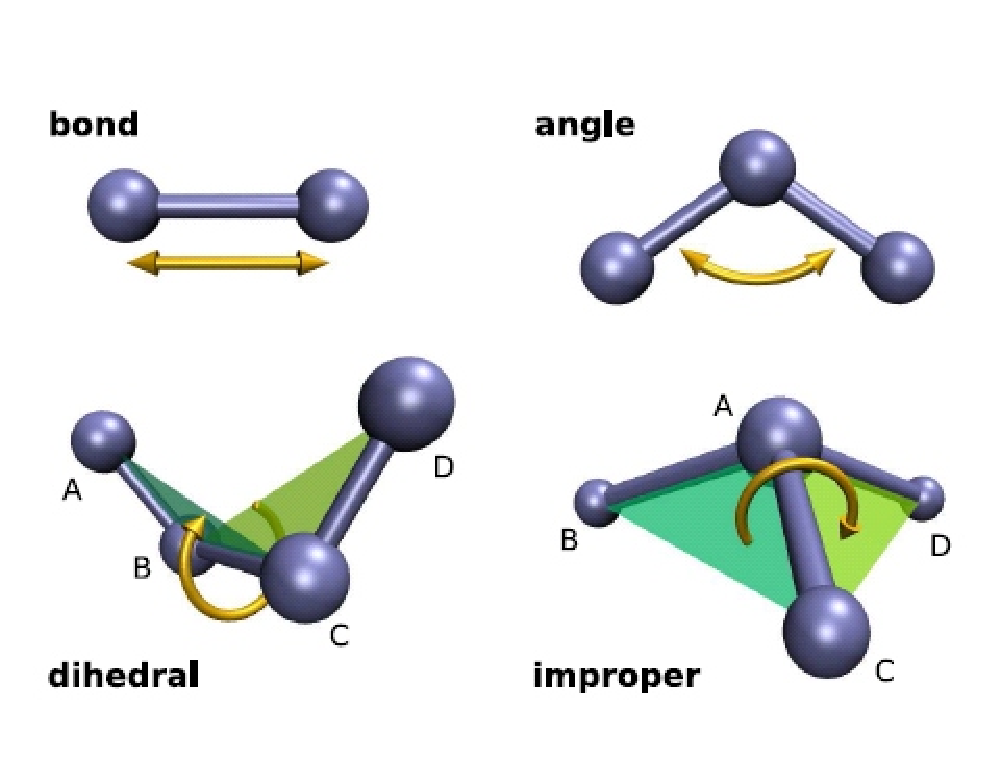
\includegraphics[scale=0.65]{Chapter3/bond1}
\caption[The various bonding between atoms and planes in a molecule.]{The various bonding between atoms and atomic planes in a molecule~\citep{Bergethon1998}.}
\label{bond1}
\end{figure} 

%%%%%%%%%%%%%%%%%%%%%%%%%
{\textbf{Bond Stretching}}:
%%%%%%%%%%%%%%%%%%%%%%%%%
The bond stretching between two bonded atoms \emph{i} and \emph{j} is represented by harmonic potential,
\begin{equation}
{\rm U}_{\rm b}(r_{ij}) =\frac{1}{2}\;k_{ij}^{\rm b}\;(r_{ij} - b_{ij})^2 
\end{equation}
where $b_{ij}$ is the bond length between two atoms and $k_{ij}^{\rm b}$ is the force constant.
%\begin{figure}[h!]
%\centering
%\includegraphics[scale=0.3]{Chapter3/bond}
%\caption{Figure at left represents the schematic diagram of Bond stretching and that at the right is its harmonic potential \cite{Gromacs-manual}.}
%\label{bond}
%\end{figure}

%%%%%%%%%%%%%%%%%%%%%%%%%
{\textbf{Bond-angle vibration}}:
%%%%%%%%%%%%%%%%%%%%%%%%% 
The change in angle between three consecutive bonded atoms (say \emph{i, j, k}) from its equilibrium value causes vibrational motion and this type of vibration is defined by angular harmonic potential. Mathematically, the expression can be written as
\begin{equation}
{\rm U}_{\rm angle}(\Theta_{ijk}) = \frac{1}{2} k_{ijk}^{\Theta}(\Theta_{ijk}- \Theta^0_{ijk})^2.
\label{vibration}
\end{equation}
Here $k^\Theta_{ijk}$ and $\Theta^0_{ijk}$ are the angular force constant and equilibrium bond angle respectively. Since the both, bond stretching and bond-angle vibration, are represented by harmonic potential their curvature seems to be similar. 

%%%%%%%%%%%%%%%%%%%%%%%%%
{\bf Proper dihedral}: 
%%%%%%%%%%%%%%%%%%%%%%%%%
Dihedral angle is based on four-body interactions. Proper dihedral is the angle between two planes made up of four consecutive atoms which constrain the rotation around a bond. In Figure ~\ref{bond1}, two planes are formed by A-B-C and B-C-D. The periodic dihedral potential can be written as, in the form of equation~\ref{proper},
\begin{equation}\label{proper}
{\rm U}_{\rm dihed} = k_{\phi} (1 + \cos(n\phi - \phi_s),
\end{equation}
%%%%%%%%%%%%%%%%%%
where $k_{\phi}$ is force constant, $n$ is multiplicity number, $\phi$ is proper dihedral angle and $\phi_s$ is the angle at which the potential attains its minimum value. The multiplicity ($n$) represents the number of minima when bond is rotated through $2\pi$. 

{\bf Improper dihedral}: Improper dihedral potential forces atoms to remain in a plane or to prevent from transition to its mirror image. Improper dihedral is also the angle between two planes formed by ABC and ACD (Figure \ref{bond1}), however, the atom A remains at the center rather than end of the one of planes in proper dihedral. The harmonic form of improper potential can be represented as,  
%%%%%%%%%%%%%%
\begin{equation}
{\rm U}_{\rm impr} = \frac{1}{2} k_\xi (\xi - \xi_{0})^2 
\label{improper}
\end{equation}
%%%%%%%%%%%%%%%%%
where $k_\xi $ is force constant, $\xi$ is improper dihedral angle and $ \xi_0 $ is equilibrium improper dihedral angle. 

{\textbf{Non- Bonded Interaction}}: Beside the bonded interactions, there are few non-bonded interactions in between the particles. Two of the main non-bonded type are Coulomb and van der Waals (vdW) interactions. In case of non-polar molecules like methane and closed shell atoms like Ar, Kr etc, usually the coulomb interaction is not present. In such a situation, potential energy of a systems is composed of short-ranged repulsive term because of overlapping electron clouds and long-ranged attractive term because of the vdW interactions. The most popular potential which incorporates these terms is called Lennard-Jones (LJ) potential \citep{Kittel2005}. LJ potential is also known as 12-6 potential and represented by,
\begin{equation}
U_{\text{LJ}}(r_{ij}) = 4\epsilon_{ij}\left[\left(\frac{\sigma_{ij}}{r_{ij}}\right)^{12} - \left(\frac{\sigma_{ij}}{r_{ij}}\right)^6\right].
\label{LJI}
\end{equation}
In equation (\ref{LJI}), $\sigma$ and $\epsilon$ are the Lennard-Jones constant, which are usually chosen via empirical methods \citep{Ercolessi1997}. In GROMACS package, these constants are already available for many atoms/systems for further applications.  

\begin{figure}[h!]
\centering
\includegraphics[scale=0.6]{Chapter3/lennard.png}
\caption[A typical Lennard-Jones potential.]{ A typical  Lennard-Jones potential for an atom. The symbols $\sigma$ and $\epsilon$ represent the repulsive region and the minimum potential at equilibrium state, respectively.}
\label{lennard}
\end{figure}

When two atoms are brought very close to each other, their electron cloud starts overlapping and causes 
partial promotion of electrons to unoccupied higher energy orbitals~\citep{Kittel2005}. Hence the energy of the system increases, and the interaction becomes repulsive. This phenomenon is described by Pauli-exclusion principle. In equation \ref{LJI}, the repulsive term is represented by the first term $({1}/{r_{ij}})^{12}$ which is obviously dominant at short distances. The second term $({1}/{r_{ij}})^6$, on the other hand, constitutes the attractive part and is dominant at large distances. As we discussed above, this is because of vdW interactions which are originated due to interactions in between electric-dipoles. The vdW interactions are the non-local type of interactions and are the consequences of three different contributions. The contributions from the interactions in between polar molecules or permanent dipoles are referred as Keesom interactions. On the other hand, the vdw interactions in between permanent dipoles and induced dipoles are related to Debye interactions~\citep{Stone1996, Ulman2014}. The most common type of non-local interactions, originated from instantaneous dipole and induced-dipole interactions where the fluctuation of electron density at one region induces dipole into another region of the system, are called London dispersion interactions~\citep{Klime2012}. The London dispersion interactions (proportional to $(1/r_{ij})^6$) is incorporated LJ potential. Although vdW is a weak and long-ranged potential, it is important in the systems with spherical valence shells (where other dominant interactions are absent)~\citep{Leach2001}.

The LJ potential can also be expressed in new parameters, (${C_{ij}}^{(12)}$ and ${C_{ij}}^{(6)}$) 
with ${C_{ij}}^{(12)}= 4\epsilon_{ij} \sigma_{ij}^{12}$ and ${C_{ij}}^{(6)} = 4\epsilon_{ij} \sigma_{ij}^6$. 
Hence equation \ref{LJI} becomes 
\begin{equation}\label{LJ}
U_{\text{LJ}}(r_{ij}) = \left[\frac{C_{ij}^{(12)}}{r_{ij}^{12} } - \frac{C_{ij}^{(6)}}{r_{ij}^6 }\right]
\end{equation}
One can use proper combination rules to calculate the parameters of molecules with different values of atomic LJ constants~ \citep{Gromacs-manual}.

%%%%%%%%%%%%%%%%%%%%%%%%%
{\textbf{Coulomb Interaction}}: 
%%%%%%%%%%%%%%%%%%%%%%%%%
Coulomb interaction may exist in between the point charges of same or different molecules. For any two
point charges $q_i$ and $q_j$ separated by distance $r_{ij}$, the coulomb term can be expressed as:
\begin{equation}
\textrm{{U}}_{\rm coulomb} = \frac{q_iq_j}{4\pi\epsilon\epsilon_or_{ij}}
\label{Coulomb}
\end{equation}
In equation (\ref{Coulomb}), $\epsilon$ and  $\epsilon_\circ$ represent the dielectric constant and the permittivity of free space, respectively. Coulomb potential has very important role in case of ionic system, and sometimes may exist in non-ionic systems when electron density in valence shells shifts due to unequal values of electronegativity of atoms.

\begin{sloppypar}
{\textbf{Periodic Boundary Conditions (PBCs)}}: Particles at/near to the surface feel different forces than that of the particles deep inside the surface(boundary) \citep{Allen1989}. Ideal infinite-systems have no surface atoms, however, the real systems are different from this hypothesis. For an example, in case of 1000 atoms in a cubical box (arranged by $10\times10\times10$), more than 488 atoms appear at the surface of the cube \citep{Allen1989}. In larger (macroscopic) systems, only a small fraction of atoms are close enough to the surface of the container to realize the surface effects (an effect due to presence of surface or wall of the container which provide rigid boundary for atoms while trying to escape during the simulation). 
\end{sloppypar}

The system-size of usual molecular dynamics is limited to few thousands of atoms because of complexity in structure and computational limitations. The smaller systems are dominated by surface effects, and one of the 
easiest ways to minimize the surface effect is to consider the periodic boundary condition where the system is surrounded by the copies of its images \citep{Frenkel2002}. It means the box containing N number of atoms (to be simulated) is assumed to be a primitive cell which is propagated through out the space to construct an infinite system. Hence the boundary of the central box has been removed and the particles feel no surface effects. During the course of simulation, when one particle leaves the box from one side, its nearby image enters into the box from another side keeping the number density of the system fixed~\citep{Hansen2006}. 
%%%%%%%%%%%%%%%%%%%%
\begin{figure}[h!]
\centering
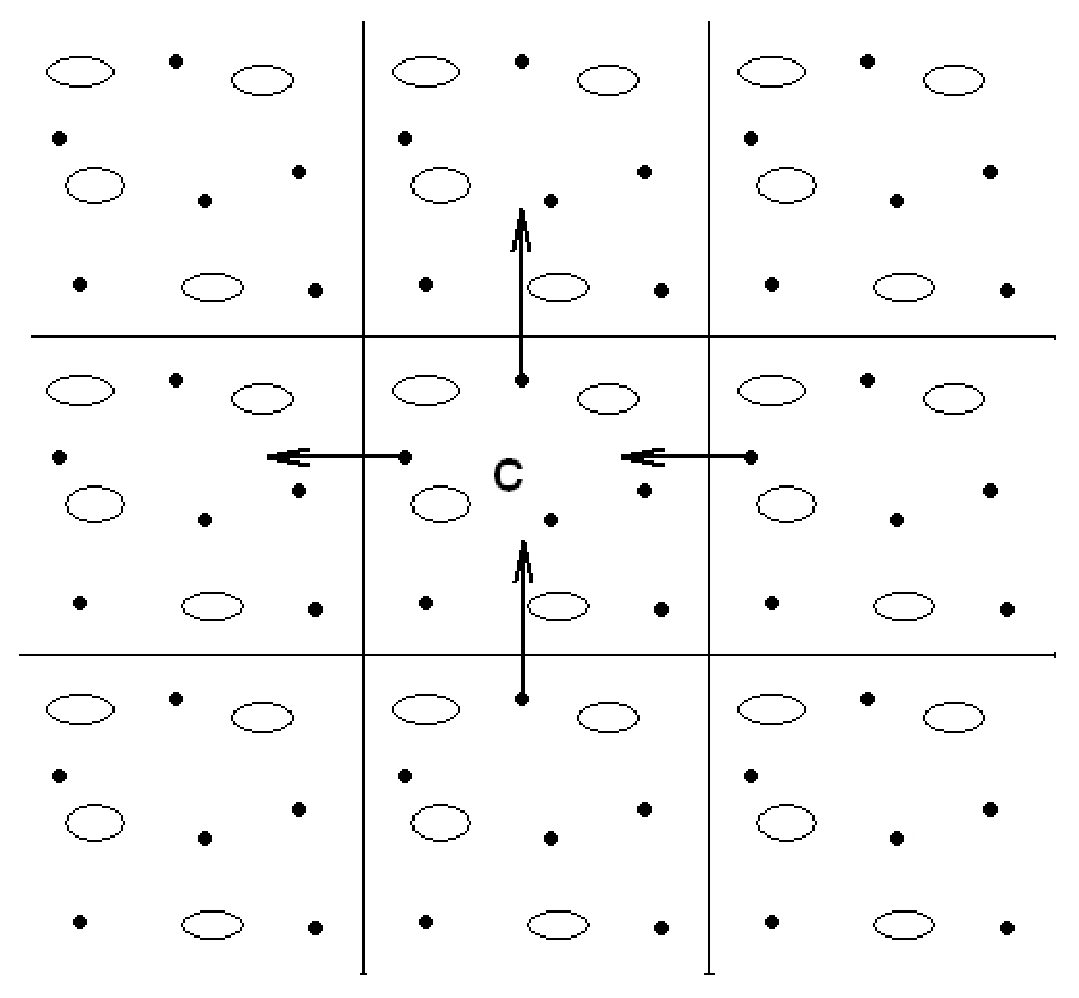
\includegraphics[scale=0.52]{Chapter3/pbc.eps}
\caption[Schematic representation of periodic boundary conditions.]{Schematic representation of periodic boundary conditions \citep{Gromacs-manual}.}
\label{pbc}
\end{figure}
%%%%%%%%%%%%%%%%%
Another consequence of PBC is {\it minimum image criterion} which is applicable to limit the interaction between the particles. That is among $N$ number of particles, each atom interacts with the closest images of other $N - 1$ particles and ignores all remaining images \citep{Allen1989}. Since the potential is considered through pairwise addition of the interactions, the total potential involves $N(N - 1)/2$ terms, which is still high and can be reduced further ( for short range interactions) by using spherical cut-off. To avoid the images from double counting, the value of cutoff (say $R_{\text{c}}$) should not be greater than half of the box size \citep{Ercolessi1997}. For long range interactions (like for ionic systems), however, truncation of potential at small $R_{\text{c}}$ can not include the interactions at longer distances and causes a serious problem. This problem can be minimized by using the method of Ewald, where short-range potential is summed in real space with appropriate truncation, and the long-range summation is taken over the reciprocal lattice vectors \citep{Hansen2006}.

Although the size effect is minimized by using PBC, it is not the absolute solution. Its magnitude depends up on the kind of the system and the properties of interest. One can check varying size samples to estimate the size effect and possible error due to chosen size~\citep{Poudyal2014}. 
%%%%%%%%%%%%%%%%%%%%%%%%%
\subsection{Initialization} \label{Initial-MD}
%%%%%%%%%%%%%%%%%%%%%%%%%
\begin{sloppypar}
Initialization is the step to assign the initial co-ordinates and velocities which should be compatible to the structures. One has to exclude the overlap of atomic cores while choosing positions in this stage. The velocities are attributed by using Maxwell-Boltzmann distribution and scaled to adjust the mean kinetic energy to the desired values \citep{Gromacs-manual}. The relationship of velocity with temperature in thermal equilibrium is given by \citep{Frenkel2002},
\end{sloppypar}
\vspace{-25pt}
\begin{equation}
\langle v_\alpha^2 \rangle = \frac{k_{\text{B}} T}{m}.
\end{equation}
Here $v_\alpha$ is the $\alpha(x,y,z)$ component of the velocity, $m$ is the mass of a given particle, $T$ is the temperature and $k_{\rm B}$ is Boltzmann's constant. 
%%%%%%%%%%%%%%%%%%%%%%%%%
\subsection{Force Calculation}
%%%%%%%%%%%%%%%%%%%%%%%%%
\begin{sloppypar}
The main step of MD simulations after {\it initialization} of a system, is the calculation of forces acting on each of the particles. This process includes the estimation of forces on a particle $i$ due to all its neighbors \citep{Ercolessi1997}. By using the relation of potential, which is pairwise addition of interacting particles ${\rm U}(r_i)$, the force can be calculated by
\begin{equation}
\mathbf{F_i} = -\nabla_i\textrm{U}(\mathbf{r}_i).
\end{equation}
Calculation of forces should include all the interacting particles within the range of defined cutoff and excludes all the remaining ones. 
The procedure follows the {\it minimum image convention} where particle $i$ interacts with the nearest image of $j$ \citep{Frenkel2002, Ercolessi1997}. \end{sloppypar}

\begin{figure}[h!]
\centering 
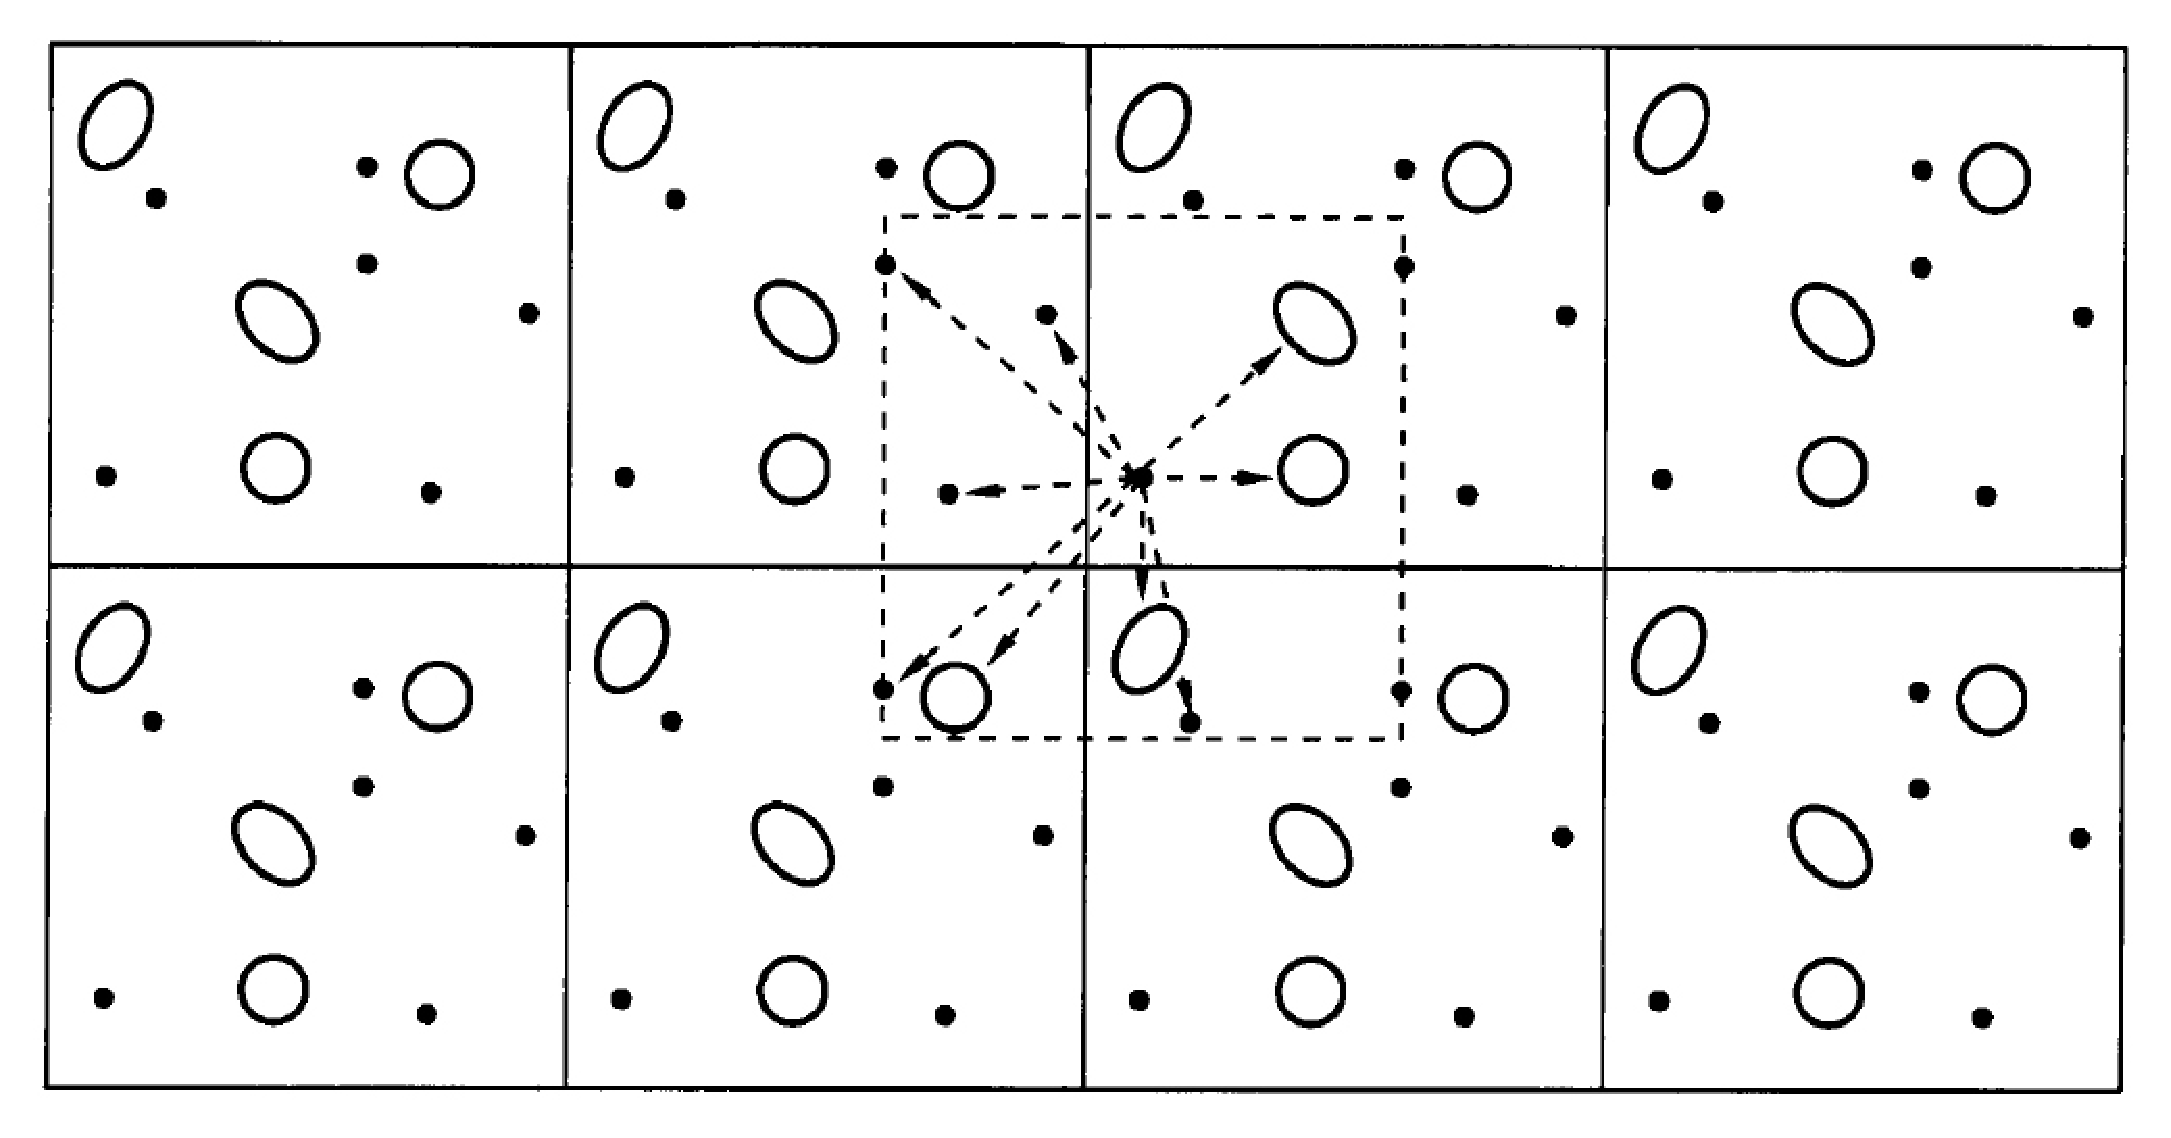
\includegraphics[scale=0.38]{Chapter3/cutoff.eps}
\label{cutoff}
\caption[Cut-off and near-image convention for periodic boundary condition. ]{Use of cut-off and near-image convention for periodic boundary condition \citep{Frenkel2002}.}
\end{figure}

The value of cutoff ${\rm R}_{\text{c}}$ can not be large enough due the limitations on the size of the simulating box 
(${\rm R}_{\text{c}}$ should not be greater than half of the box-size). For long range interactions, however, the interaction beyond ${\rm R}_{\text{c}}$ could be significant and needs correction. One of corrections is based on mean field approximation where the field beyond ${\rm R}_{\text{c}}$ is constant \citep{Thapa2013}. Another usual method for the correction includes Ewald summation in which all interactions between the particle {\it i} in the central cell and its (unit cells) replica surrounding the central one are integrated~\citep{Gromacs-manual}.
%%%%%%%%%%%%%%%%%%%%%%%%%
\subsection{Integration of Equation of Motion}
%%%%%%%%%%%%%%%%%%%%%%%%%
The calculations of new coordinates for position and components of velocities of particles by using their initial (known) information is related to the solution of equations of motion. The forces are position dependent through potentials, and mathematical algorithms are able to predict the new coordinates by using the available information. Hence the phase space coordinates generate their trajectories. There are many methods to trace these trajectories, and the methods with higher precision with the least possible computational cost are supposed to be the most preferred ones. The precision and computational cost are contradictory for a simulation, and requires compromise in between their perfect conditions\citep{Allen1989}. In case of MD simulations, the length of time step is one of the major determining factors for computational cost (the higher the time step, 
the lesser the computational cost) and accuracy (the smaller the time step, the higher the accuracy).
%%%%%%%%%%%%%%%%%%%%%%%%%
\subsection{Verlet Algorithm}
%%%%%%%%%%%%%%%%%%%%%%%%%
\begin{sloppypar}
One of the popular methods for integrating the equations of motion is Verlet algorithm where the positions $\textbf{r}(t)$, and
accelerations $\textbf{a}(t)$ are found from the previous steps~\citep{Frenkel2002}. The relations for Verlet algorithm are based on Taylor series expansion, by using which for the time step $\delta t$ we get 
\end{sloppypar}
\vspace{-20pt}
\begin{align}
\textbf{r}(t+\delta t) & = \textbf{r}(t) + \textbf{v}(t) \delta t + \frac{\textbf{F}(t)}{2 m} \delta t^2 + \frac{\delta t^3}{3!} \frac{d^3 r}{d t^3} + O(\delta t^4) \label{ver1} \\
\textbf{r}(t-\delta t) & = \textbf{r}(t) - \textbf{v}(t) \delta t + \frac{\textbf{F}(t)}{2 m} \delta t^2 - \frac{\delta t^3}{3!} \frac{d^3 r}{d t^3} + O(\delta t^4) \label{ver2}
\end{align}
Now adding equations (\ref{ver1}) and (\ref{ver2}) we get 
\begin{align}
\textbf{r}(t+\delta t) + \textbf{r}(t-\delta t) = 2 \textbf{r}(t) + \frac{\textbf{F}(t)}{m} \delta t^2 + O(\delta t^4) \\
\textbf{r}(t+\delta t) = 2 \textbf{r}(t)-\textbf{r}(t-\delta t) + \frac{\textbf{F}(t)}{m} \delta t^2 + O(\delta t^4)
\label{ver3}
\end{align}
Equation (\ref{ver3}) shows that error in position is in the order of $\delta t^4$. Velocities are importat to estimate the kinetic energy (however are absent in position trajectories), and can be obtained by using equations
(\ref{ver2}) and (\ref{ver1}). 
\begin{align}
& \textbf{r}(t+\delta t) - \textbf{r}(t-\delta t) = 2 \textbf{v}(t) \delta t + O(\delta t^3) \\
\label{verlv}
& \textbf{v}(t) = \frac{\textbf{r}(t+\delta t) -\textbf{r}(t-\delta t)}{2 \delta t} - O(\delta t^2) 
\end{align}
Since the error of velocity is in the order of $\delta t^2$ (comparing to $\delta t^4$ in positions), accuracy 
is expected to be lower in velocity. Furthermore, velocity and positions could not be calculated simultaneously, 
that is velocity at time t needs the coordinates at $t+\delta t$. 

\subsection{Leap frog Algorithm}
Leap frog algorithm  is an equivalent scheme to Verlet algorithm. It is named for half-integer time steps of velocities with respect to positions (and acceleration), and uses these velocities to compute the new positions. 
It means that velocities leap over the position coordinates to give the next mid step values (Figure~\ref{leap_frog}) ~\citep{Frenkel2002}. If $(t-\delta t/2)$ and $(t+\delta t/2)$ are the mid-integer time steps, the corresponding velocities are defined by
%%%%%%%%%%%%%%%%%%%%%
\begin{equation}
\textbf{v}\left(t-\frac{\delta t}{2}\right) \equiv \frac{\textbf{r}(t)-\textbf{r}(t-\delta t)}{\delta t}
\label{v-minus}
\end{equation}
and \begin{equation}
\textbf{v}\left(t+\frac{\delta t}{2}\right) \equiv \frac{\textbf{r}(t + \delta t) - \textbf{r}(t)}{\delta t}\,.
\label{v-plus}
\end{equation}
%%%%%%%%%%%%%%%%%%%%
The new positions can be calculated from  the old positions and velocities. 
\begin{equation}
\textbf{r}(t+\delta t) = \textbf{r}(t) + \textbf{v}\left(t+\frac{\delta t}{2}\right) \delta t  
\end{equation}
%%%%%%%%%%%%%%%%%%
By using the Taylor series expansion on velocity about $t$, we get the Verlet type relations as
\begin{equation}
\textbf{v}\left(t+\frac{\delta t}{2}\right) = \textbf{v}(t) + \frac{\textbf{F}(t)}{2 m} \delta t\, .
\end{equation}
Again,
\begin{equation}
\textbf{v}\left(t-\frac{\delta t}{2}\right)= \textbf{v}(t) - \frac{\textbf{F}(t)}{2 m} \delta t\, .
\end{equation}
Solving the above two equations we get
\begin{equation}\label{leap_v}
\textbf{v}\left(t+\frac{\delta t}{2}\right) = \textbf{v}\left(t-\frac{\delta t}{2}\right) + \frac{\textbf{F}(t)}{m} \delta t\, .
\end{equation}
Since the velocities and positions are defined at different time, potential energy and kinetic energies can not be defined simultaneously. It means the total energy can not be calculated directly from the above equations. However, the trajectories for the position and velocities are similar~\citep{Ercolessi1997, Bergethon1998}. The schematic representation of Leap frog algorithm is shown in Figure \ref{leap_frog}.

\begin{figure}[h!]
\centering
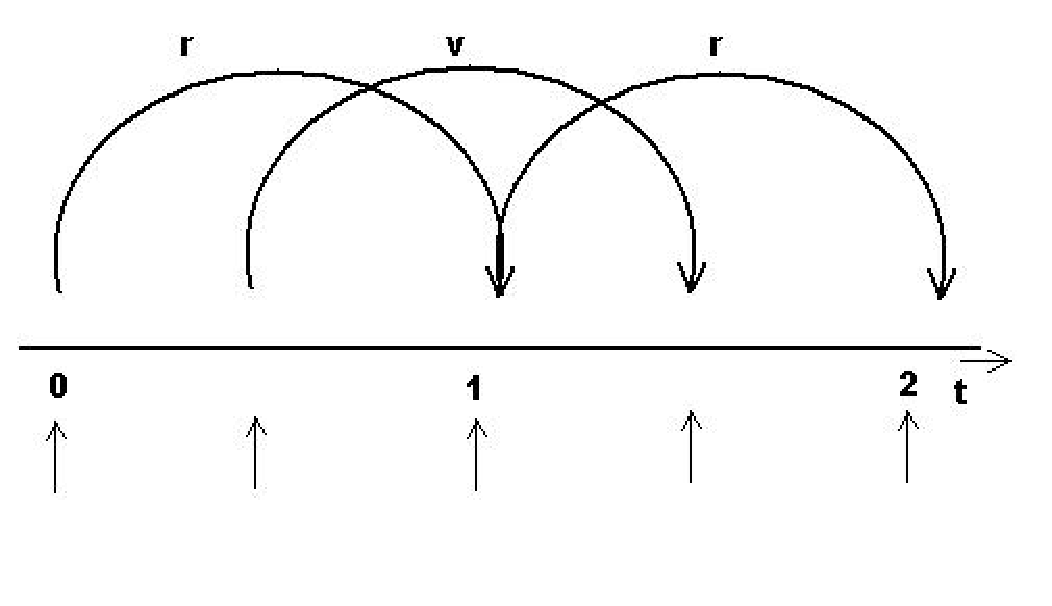
\includegraphics[scale=0.40]{Chapter3/leapfrog.eps}
\caption[Schematic representation of leap-frog algorithm. ]{Schematic representation of leap-frog algorithm \citep{Frenkel2002}.}
\label{leap_frog}
\end{figure}
Time reversibility is one of the major applications of leapfrog integration. It means integration for n steps forward, and then $n$ steps backwards bring the system at the starting (same) position~\citep{Allen1989}. 
The velocities at current time {\it t} can also be calculated via indirect method (by using equations \ref{v-minus} and \ref{v-plus}), 
\begin{equation}
\textbf{v}(t) = \frac{1}{2} \left(\textbf{v}\left(t + \frac{1}{2} \delta t\right) + \textbf{v} \left(t - \frac{1}{2} \delta t\right)\right)\,.
\end{equation}
\subsection{Constraint Dynamics}
The non-polar spherical atoms can be treated with the LJ potential which used to be the obvious choices in early 
MD simulations \citep{Harp1968, Harp1970}. In molecular systems, however, the fundamental particles interact with intra- and intermolecular forces which are accounted by bond vibrations and changes in relative orientation etc. Some of these vibrations are very fast and require extremely short time step. This complexity in simulations can be replaced by constraint dynamics where the intra-molecular bonds and angles are supposed to be fixed. The magnitude of vibrations are small comparing to their molecular dimensions, and this assumption is near to the reality. For such a purpose, we need a constraint to force the system into required rigidities \citep{Leach2001}. SHAKE and LINCS are two popular constraints available in GROMACS package.  In the present work, we have used SHAKE as constraint algorithm where a set of unconstrained co-ordinates are changed to another set that are constrained with distances~\citep{Gromacs-manual}.
%%%%%%%%%%%%%%%%%%%%%%%%%
\section{ Statistical Ensembles in Molecular Dynamics}
%%%%%%%%%%%%%%%%%%%%%%%%%
The dynamical state of any system (having $N$ number of particles) is defined by $3N$ position and $3N$ momentum coordinates. A set of these $6N$ variables define a micro-state in $6N$ dimensional phase space which is called phase point. We introduce {\it ensemble} to explain the probability distribution of the microscopically defined states of a system in terms of imaginary collections of the system. Each of these collections is the replica of real systems with same macroscopic properties. The concept of such ensembles realize the physical observables in terms of their average values~\citep{pathria1996}.

Depending up on the variables kept fixed in the systems, ensembles are classified as microcanonical (NVE), canonical (NVT), isothermal-isobaric (NPT) and grandcanonical ($\mu$VT) ensembles. The symbols refer to the number of particles (N), volume (V), energy (E), pressure (P) and temperature (T) and the combination of these variables define the type of ensemble. Constant temperature, and constant pressure experiments respectively, are relevant to NVT and NPT ensembles. Microcanonical (NVE) ensembles are very common in MD simulations. Upon 
having enough lapse of time in MD simulations time average of desired properties like: total energy, can be replaced by ensemble averages (average property of large number of replications of systems at a time) which simplifies calculating the properties of interest. Such a condition where the time average of an observable in a system is equivalent to the ensemble average, is called ergodic \citep{Leach2001}. 

In MD simulations, pressure and temperature vary a lot. To fix them, some regulatory mechanisms are required \citep{Leach2001}. For the purpose of controlling temperature (T) and pressure (P), we have different coupling systems, and some of them are described in the following paragraphs. 
%%%%%%%%%%%%%%%%%%%%%%%%%
\subsection{Temperature Calculation and Control} \label{thermostat}
%%%%%%%%%%%%%%%%%%%%%%%%%
The initial particle velocities in a system are defined by Maxwell-Boltzmann distribution as described in section~\ref{Initial-MD}. During the course of simulation, however, the velocity distribution changes to new values. Since the velocities are correlated with the kinetic temperature of the system, they need to be rescaled according to the target temperature which is the requirement for constant temperature ensembles. The ensembles with constant temperature are either NVT or NPT. The constant temperature condition is also the fundamental requirement for correct ensemble averages to study the properties of the system as a function of temperature like folding and unfolding  of proteins \citep{Leach2001}. The temperature-controlled simulations are also important in order to systematically increase or decrease the temperature of the system like for simulated annealing. The correct temperature, within reasonable fluctuations, is maintained by using different types of temperature-control mechanisms like rescaling the velocities or by external heat baths (thermostats) \citep{Frenkel2002}. The choice of the thermostat depends on the nature of system and the properties of interest. Berendsen thermostat is useful for the cases of weak coupling scheme \citep{Berendsen1984} and the extended-ensemble approach is attained by Nose-Hoover thermostat \citep{Nose1984, Hoover1985}. We have used velocity-rescale (v-rescale) type of thermostat for such purpose. Velocity-rescale thermostat is basically identical with the Berendsen thermostat except few extra terms which ensure a correct kinetic energy distribution~\citep{Gromacs-manual}.

Rescaling velocities to control the temperature are related through the time average kinetic energy of the system, $\left\langle \text{K.E.} \right\rangle = \frac{3}{2} k_{\rm B}T$, with some rescaling factor, $\lambda = [ {\rm T}_{\rm new}/{\rm T}(t) )^{1/2}]$. Here ${\rm T}_{\rm new} $ and $ {\rm T}(t) $ are new temperature after rescaling velocities and temperature at time $ t $ respectively.

Heat baths, on the other hand, exchange heat with the system to attain the target temperature.  
\begin{equation}\label{thermo}
\frac{d{\rm T}(t)}{dt}  =  \frac{1}{\tau} ( {\rm T}_{\rm bath} - {\rm T}(t)),
\end{equation}
where $\tau$, ${\rm T}_{\rm bath}$ and T($t$) represent the coupling constant, target (bath) temperature and the temperature at time $t$ respectively.

In the microcanonical ensemble (constant NVE), temperature is defined by making use of the equipartition principle which states that the average kinetic energy per degree of freedom is $\frac{k_{\rm B}{\rm T}}{2}$. The instantaneous temperature in such a system becomes  
\begin{equation}
{\rm T}(t) = \frac{2}{(3N - N_{\text{c}})k_{\rm B}}\sum_j^N\frac{1}{2}m_iv_i^2(t)
\end{equation}
Here ${N}$ and ${N}_{\text{c}}$ represent the number of particles and number of constraints on the system, respectively. Similarly, $m_i$ and $k_{\rm B}$ represent mass of the $i^{\rm th}$ particle and Boltzmann's constant respectively.
%%%%%%%%%%%%%%%%%%%%%%%%%
\subsection{Pressure calculation and control}
%%%%%%%%%%%%%%%%%%%%%%%%%
As similar to the constant temperature, constant pressure simulations are important in many practical cases. The experiments at constant pressure are very common and computational work at similar condition is relevant for the purpose of estimation and comparison with the experiments. At fixed temperature (see subsection~\ref{thermostat}), NPT ensemble is characterized by constant pressure and number of particles. In practice, constant pressure simulations are  important to study the system-properties as a function of pressure such as pressure induced phase transitions \citep{Leach2001}. 

Since the constant pressure is usually maintained by changing volume, the observation of fluctuations in volume are important. NPT system is related to isothermal compressibility with the relation
\begin{equation}
\kappa  = - \frac{1}{V} \frac{{\partial}{\rm V}}{{\partial} {\rm P}} .
\end{equation}
This indicates that the easily compressible substance has larger changes/fluctuations in volume, comparing to the incompressible substances. In the reverse way, less compressible substance has larger fluctuations in pressure at constant volume. As similar to the control in temperature, there are various schemes to control pressure. They could be either by scaling the volume or by using pressure bath (barostats) \citep{Gromacs-manual}, 
\begin{equation}
\frac{\d{\rm P}(t)}{\d t}  =  \frac{1}{\tau_p} ( {\rm P}_{\rm bath} - {\rm P}(t)). 
\label{baro}
\end{equation}
\begin{sloppypar}
In the equation (\ref{baro}), $\tau _p$, ${\rm P}_{\rm bath}$ and P($t$) represent the coupling constant, target (bath) pressure and the pressure at time $t$ respectively. Pressure is felt by the momentum carried out by the particles while they cross the boundary and the force of interaction in between the particles at different surfaces. There are different types of barostats to control the pressure inside a simulation box, which are described in available literature~\citep{Parrinello1981, Melchionna1993, Andersen1980}. In the present work, 
we have used Parrinello-Rahman type of barostat for such a purpose. In Parrinello-Rahman Barostat, box-vectors follow an equation of motion where the equation of motion of the particles are also changeable. This type of barostat can also be applied in varying shapes of simulation cells~\citep{Parrinello1981}.
\end{sloppypar}

\begin{figure}[h!]
\centering
\includegraphics[scale=0.55]{Chapter3/MD_flowchart.png}
\caption{A typical molecular dynamics simulation flow chart representation.}
\label{md_flow}
\end{figure}

Flow chart (Figure \ref{md_flow}) shows that the construction of correct topology file is the first step of the simulation process. This can be done by using the coordinate file of the system via proper GROMACS executable (pdb2gmx). The choice of right size of the box and the number of solvent molecules are the next steps of the simulation which need care of nature of interactions and minimum image criteria. According to this convention, the separation between the molecules can not be greater than the half of the box size. In the process of minimization, the system finds its structure and configurations corresponding to local minimum searched by the appropriate algorithm (gradient of potential is zero in such points)~\citep{Gromacs-manual}. Minimization removes the bad contacts caused by the improper position of the atoms and avoids being far from the equilibrium configuration.
%...............................................................................................
%%%%%%%%%%%%%%%%%%%%%%%%%
\section{Systems under study}
%%%%%%%%%%%%%%%%%%%%%%%%%
In the present work, transport properties, diffusivity of methane and other three light alkanes, NO, CO, N2,  diffusivity and mobility of halide and alkali ions in water, and thermodynamic properties, free energy of solvation of methane, ethane, propane and n-butane in water and methanol  are studied.
%%%%%%%%%%%%%%%%%%%%%%%%%
\subsection{Methane and various gases in water} \label{methane_diffusion}
%%%%%%%%%%%%%%%%%%%%%%%%%
\begin{sloppypar}
Alkanes are saturated hydrocarbons that consist only of the elements carbon (C) and hydrogen (H), where each of these atoms are linked together exclusively by single bonds. The smaller members of the alkane family are gases, while the larger are liquid and solid compounds. First four members (lighter alkanes) of alkane series are methane, ethane, propane, and butane with molecular formula $\mathrm{CH_4}$, $\mathrm{C_2H_6}$, $\mathrm{C_3H_8}$, and $\mathrm{C_4H_{10}}$ respectively. Some of the common uses of them are are heating, electricity generation, cooking, production of polymers, serves as intermediate in the synthesis of drugs, pesticides and other chemicals. They are also used as propellants in aerosol sprays and   have a number of industrial applications beyond fuels, including uses in cosmetics and plastics \citep{morrison2011, brown2014introduction}. Furthermore, the first four members of alkanes are also neutral analogs of amino acid side chain. Amino acid side chain analogs represent a natural test case for biomolecular interaction~\citep{shirts2003extremely, shirts2005solvation}.
\end{sloppypar}

The SPC/E ( simple point charge/extended) potential  model~ \citep{berendsen1987missing} is used in all the simulation for water as a solvent. The OPLSS-AA (Optimized Potentials for Liquid Simulations-All Atom) potential model~ \citep{kaminski2001evaluation}  is used for alkanes (methane, ethane, propane, n-butane) as  solute. The forcefield parameters (bonded and non-bonded)  used to parametrize the other  studied system including alkanes and water, carbon monoxide molecule~\citep{kowalczyk2012molecular, banwell1994fundamentals}, nitrogen molecule~\citep{atkins2009quanta, bouanich1992site}, and NO molecule~\citep{zhou2005molecular} are is presented in table(\ref{bonded}) and table(\ref{non-bonded}). In classical force fields like OPLS-AA, the potential functions are derived empirically to describe the atomic interactions. The atoms are treated as spherically symmetric particles and are considered to be connected through covalent bonds to form molecules. Each and every atom experiences a force resulting from its pairwise additive interactions with the rest of the system. The total potential energy $\mathrm{U_{tot}}$  includes contributions from both bonded and  non-bonded interactions  \citep{Gromacs-manual}. The bonded interactions are bond stretching (2-body), bond angle (3-body) and dihedral angle (4-body) interactions. A special type of dihedral interaction (called improper dihedrals) is used to force atoms to remain in a plane or to prevent transition to a configuration of opposite chirality (a mirror image). The non-bonded   interactions are represented by the Lennard-Jones potential  and Coulomb potential. 

The systems under study consist of $3$ alkane (methane, ethane, propane, n-butane) molecules and 971 water molecules,  $5$ NO molecules and 280 water molecules,  $5$ CO molecules and 280 water molecules  $5$ N2 molecule and 265 water molecules separately as different sytems. In this study, we have used  the following  dihedral potential (Ryckaert-Bellmans potential)~ \citep{Gromacs-manual} for alkanes:   
\begin{equation}
U_{\text{RB}} = c_0 + c_1(1+ cos\phi)  + c_2(1- cos2\phi) + c_3 (1+ cos3\phi) 
\end{equation}
where $\mathrm{\phi}$ is the dihedral angle and $\mathrm{c_0, c_1, c_2, c_3}$ are constants.

The non-bonded interatomic interaction is the sum of Lennard- Jones interaction ($\mathrm {U_ {LJ}}$)  and Coulomb interaction ($\mathrm {U_ {Coul}}$), that can be written as:
\begin{equation}
U_{\alpha\beta}(r_{ij}) = 4\epsilon_{\alpha \beta}\left[\left(\frac{\sigma_{\alpha\beta}}{r_{ij}}\right)^{12} - \left(\frac{\sigma_{\alpha\beta}}{r_{ij}}\right)^6\right] +  \frac{q_{i\alpha}\;q_{j\beta}}{4\pi\epsilon_0\;r_{ij}}
\end{equation}
 where $r_{ij}$ is the Cartesian distance between the two atoms $i$ and $j$; $\alpha$ and $\beta$  indicate the type of the atoms

\begin{table}[H]
\centering
\caption [Force-field (bonded) parameters for SPC/E water, OPLS-AA Alkanes, NO, CO and N2.] {Force-field (bonded) parameters for SPC/E water, OPLS-AA Alkanes, NO, CO and N2. The units of  equilibrium bond length ($b$) and equilibrium bond angle ($\Theta^0$) are  nanometer (nm) and degrees ($^o$) respectively. Similarly, the units of  $k^b$, $k^{\Theta}$ and $\mathrm{c_i}$ ($\mathrm{c_0}$, $\mathrm{c_1}$, $\mathrm{c_2}$, $\mathrm{c_3}$) are $\mathrm{kJmol}^{-1}\mathrm{nm}^{-2}$,  $\mathrm{kJ mol}^{-1} \mathrm{rad}^{-2}$ and  $\mathrm{kJ mol}^{-1}$ respectively. }
\label{bonded}
\resizebox {0.8\textwidth }{!}{%
\begin{tabular}{c c c c c} \hline
 \hline
SPC/E& $k^b_{\mathrm{OH}}$ & $ 345000.0$ & $b_{\mathrm{OH}}$ & 0.1000  \\ 
$\mathrm{H_2O}$ &  $k^{\Theta}_{\mathrm{HOH}}$ & $ 383.0$   & $\Theta^0_{HOH}$ & $109.47$ \\\hline
& $k^b_{\mathrm{CH}}$ & $284512.0$ & $b_{\mathrm{CH}}$ & 0.1090  \\ 
& $k^b_{\mathrm{CC}}$ & $224262.4$ & $b_{\mathrm{CC}}$ & 0.1529 \\
OPLS-AA &  $k^{\Theta}_{\mathrm{HCH}}$ & $ 276.144$   & $\Theta^0_{\mathrm{HCH}}$ & $109.47$ \\
Alkanes & $k^{\Theta}_{\mathrm{HCC}}$ & $ 313.800$ & $\Theta^0_{\mathrm{HCC}}$  & $109.47$ \\
 & $k^{\Theta}_{\mathrm{CCC}}$ & $ 488.273 $ & $\Theta^0_{\mathrm{CCC}}$ & $109.47$ \\ \hline
 & &Dihedral  (Torsional)    Potential (Alkanes)& \\ 
   H-C-C-H & $\mathrm{c_0}$ & $0.62760 $ & $\mathrm{c_1}$ & $ 1.88280$\\
 & $\mathrm{c_2}$ & $ 0.00000$ & $\mathrm{c_3}$ & $-2.51040$\\          
  H-C-C-C & $\mathrm{c_0}$ & $0.62760 $ & $\mathrm{c_1}$ & $ 1.88280$\\
 & $\mathrm{c_2}$ & $ 0.00000$ & $\mathrm{c_3}$ & $-2.51040$\\         
  C-C-C-C & $\mathrm{c_0}$ & $ 2.92880 $ & $\mathrm{c_1}$ & $-1.46440$\\
 & $\mathrm{c_2}$ & $ 0.20920 $ & $\mathrm{c_3}$ & $ -1.67360$\\  \hline
 NO & $k^b_{\mathrm{NO}}$ & $ 138092.0$ & $b_{\mathrm{NO}}$ & 0.1150  \\\hline
 CO & $k^b_{\mathrm{CO}}$ & $ 1114200.0$ & $b_{\mathrm{CO}}$ &  0.1128 \\ \hline
 N2& $k^b_{\mathrm{N2}}$ & $1380000.0$ & $b_{\mathrm{N2}}$ & 0.10975 \\ \hline \hline
\end{tabular}}
\end{table}
 \begin{table}[H]
\centering
\caption [Force-field (non-bonded) parameters for SPC/E water, OPLS-AA Alkanes, NO, CO and N2.] {Force-field (non-bonded) parameters for SPC/E water, OPLS-AA Alkanes, NO, CO and N2.}
\label{non-bonded}
\resizebox {0.60\textwidth }{!}{%
\begin{tabular}{c c  c c c}\hline \hline
& Atoms &  $\sigma$ (nm) &  $\epsilon$ (kJ/mol) &   charge (q)   \\ \hline 
SPC/E& $\mathrm{OW}$ & 0.316557 & 0.650194 & -0.8476~e  \\
Water & $\mathrm{HW}$ & 0.00000  & 0.00000 & +0.4238~e  \\\hline
& $ \mathrm{C(CH_4)}$ & 0.35000 & 0.276144  & -0.240~e \\ 
OPLS-AA & $\mathrm{C(CH_3)}$ & 0.35000 & 0.276144  & -0.180~e \\  
Alkanes &	$\mathrm{C(CH_2)}$ & 0.35000 & 0.276144  & -0.120~e \\ 
& $\mathrm{H}$ & 0.25000 & 0.125520 & +0.060~e  \\ \hline
NO & $\mathrm{N}$ & 0.3014 & 0.660977 & +0.0288~e  \\
 & $\mathrm{O}$ & 0.2875  & 0.805904 & -0.0288~e  \\\hline
CO& $\mathrm{C}$ & 0.349 & 0.189468 & +0.0203~e   \\
 & $\mathrm{O}$ & 0. 313  & 0.527685 & -0.0203~e   \\\hline
N2& $\mathrm{N}$ & 0.32920 & 0.309192 & 0.0000~e  \\\hline\hline
 \end{tabular}}
\end{table}
\noindent Here OW and HW represent the oxygen and hydrogen atoms of the water molecules respectively and $ \mathrm{C(CH_4)}$, $ \mathrm{C(CH_3)}$ and  $ \mathrm{C(CH_2)}$ are the methane, methyl and methylene carbon atoms of the alkane molecules respectively. The parameters for the non-bonded Lennard-Jones interaction between two different atoms for OPLS-AA force field  are written as~ 
 \citep{Gromacs-manual}: 
\begin{eqnarray} 
\mathrm{\sigma}_{\alpha\beta} =  \left(\mathrm{\sigma}_{\alpha\alpha} \times \mathrm{\sigma}_{\beta\beta} \right)^{\frac{1}{2}}\\
\mathrm{\epsilon}_{\alpha\beta} = \left(\mathrm{\epsilon}_{\alpha\alpha} \times \mathrm{\epsilon}_{\beta\beta} \right)^{\frac{1}{2}} 
\end{eqnarray}

MD simulation was carried out in a cubic box  with periodic boundary conditions ~ \citep{Allen1989} using \textbf{GROMACS 4.6.5}~\citep{van2005gromacs, hess2008gromacs}. The distance to the edge of the box from the solute (alkane) is an important parameter for defining the size of the box. Since we are  using periodic boundary conditions, we must satisfy the minimum image convention. That is  solute should never see its periodic image, otherwise the forces calculated will be spurious. The size of the box defined here  is sufficient for just about any cutoff scheme commonly used in simulations. After solvation, addition of  water molecules and solute (alkanes, NO, CO, N2) molecules in simulation box, energy minimization is carried out with a suitable cut off restriction depending on the size of the box, and studied system (0.9 nm-1.2 nm) to avoid unphysical van der Waals contact caused by the atoms that are too close~ \citep{Gromacs-manual}. Energy minimization brings the system to equilibrium configuration, removes all the kinetic energy from the system, reduces thermal noise in structure and brings the system to one of the local minimum. Steepest descent algorithm has been used for energy minimization and the algorithm stops when the maximum of absolute value of force components is smaller than the specified value~ \citep{Gromacs-manual}. 

 After energy minimization, isobaric-isothermal (NPT) equilibration was carried out at different temperature ranges  K and a pressure of $10^5$ N$m^{-2}$ by using \emph{velocity-rescaling} thermostat~ \citep{bussi2007canonical} and Berendsen barostat \citep{Berendsen1984}  at a coupling time $\tau_t$ = 0.01 ps and $\tau_p$ = 0.8 ps respectively. We used MD integrator~\citep{hockney1974quiet} with time step size 2 fs for  $10^9$ steps, which makes equilibration run of 200 ns. The velocity is generated initially according to a Maxwell distribution function at a specified temperature \citep{Gromacs-manual}. All the bonds are converted to constraints using SHAKE algorithm~ \citep{ryckaert1977numerical}. During equilibration short range coulomb interaction and Lennard Jones interaction each with a cut off parameter of 1.0 nm were considered  with periodic boundary conditions\citep{Allen1989}. The long range Coulomb interaction is handled via the PME (Particle Mesh Ewald) algorithm~ \citep{darden1993particle, essmann1995smooth} with fourier spacing 0.12. We monitored the temperature, pressure, density, and energy of each studied system to bring it in  thermodynamic equilibrium because dynamic property like diffusion coefficient varies with
such parameters.  After equilibration run we perform the production run to calculate the equilibrium properties of the system such as diffusion
coefficient by fixing the number of particles, volume and temperature i.e.~ NVT ensemble. We use \emph{velocity-rescale} thermostat for this
case. We don't couple the system to a fixed pressure and use the structure obtained after equilibration run by which we fix the volume of the system. The production run was carried out for 100 ns with the time step of 2 fs.

\begin{figure}[h!]
\begin{center} 
\subfigure[Methane in water]{\includegraphics[trim=1.8cm 1.8cm 1.8cm 1.8cm, clip=true, width= 7 cm]{Chapter3/structuremethane.png}}
\subfigure[Nitricoxide in water]{\includegraphics[trim=2cm 2cm 2cm 2cm, clip=true, width= 7 cm ]{Chapter3/structureNO.png}}
\end{center}
\caption[Three methane molecules and five nitric-oxide molecules  in water (H-O-H).]{ (a) Methane and (b) nitric oxide molecules in water. The shape of the box was always cubic, however, its size for the particular liquid was chosen upon the requirement of molecular size by keeping possible interaction range and minimum image criteria in mind.}
\label{methane-niticoxide}
\end{figure}
%%%%%%%%%%%%%%%%%%%%%%%%%
\subsection{Diffusivity and mobility of alkali and halide ion in water}
\label{halide_diffusion}
%%%%%%%%%%%%%%%%%%%%%%%%%
\begin{sloppypar}
The alkali metal cations $Na^+$, $K^+$  and
halide anions $F^-$, $Cl^-$, $Br^-$,$I^-$  are described by the OPLSS-AA (Optimized Potentials for Liquid Simulations-All Atom) potential model ~ \citep{kaminski2001evaluation}, while water is modeled by
TIP3P (Transferable Intermolecular Potential with 3-Points) model~\citep{jorgensen1983comparison}. In classical force fields like OPLS-AA, the potential functions are derived empirically to describe the atomic interactions. The atoms are treated as spherically symmetric particles and are considered to be connected through covalent bonds to form molecules. Each and every atom experiences
a force resulting from its pairwise additive interactions with the rest of the system. The simulation has been carried out using molecular dynamics simulation package \textbf{GROMACS} (\textbf{GRO}ningen \textbf{MA}chine for \textbf{C}hemical \textbf{S}imulation) \textbf{5.1.1}. 
 The bonded parameters for water~\citep{jorgensen1983comparison} are given in the table (\ref{bondend}).
\begin{table}[H]
\centering
\caption [Force-field (bonded) parameters for for TIP3P water.]{Force-field (bonded) parameters for TIP3P water.}
\label{bondend}
\resizebox {0.80\textwidth }{!}{%
\begin{tabular}{c c c c}\hline\hline
& Force Constant & Equilibrium bond length&\\ 
&                &      and angle&\\

$K_{\mathrm{OH}}$ & $ 5.02416 \times 10^5 \;\mathrm{KJmol}^{-1}\mathrm{nm}^{-2}$ & $b_{\mathrm{OH}}$ & 0.09572 nm \\ 
$K_{\mathrm{HOH}}$ & $ 6.2802 \times 10^2\; \mathrm{KJ mol}^{-1} \mathrm{rad}^{-2}$ & $\Theta_0$ & $104.52^o$\\ \hline
\end{tabular}}
\end{table}
 In table (\ref{bondend})  $b_{\mathrm{OH}}$  and $\Theta_0$ are the equilibrium bond length (O-H) and  the equilibrium bond angle(HOH) in water molecule respectively.  $K_{\mathrm{OH}}$  and $K_{\mathrm{HOH}}$ are the force constants of the bonds  O-H  and the strength of the bond angle vibration potential in water molecules  respectively. 
 
 The non-bonded parameters for ions~\citep{kaminski2001evaluation} and water~ \citep{jorgensen1983comparison} is given in the table (\ref{non-bondend}).
 
\begin{table}[H]
\centering
\caption[Force-field (non-bonded) parameters for ions and TIP3P water.]{Force-field (non-bonded) parameters for ions (halide and alkali) and TIP3P water.}
\label{non-bondend}
\resizebox {0.80\textwidth }{!}{%
\begin{tabular}{c c  c c c}\hline \hline
 Ions/water &  $\sigma$ (nm) &  $\epsilon$ (kJ/mol) &   charge (q)  & Ref. \\ \hline 
 $\mathrm{Na^+}$ & 0.333045   & $1.15980\times 10^{-2}$  & +1~e  & \citep{koneshan1998friction}  \\ 
 $\mathrm{K^+}$ & 0.493463 & $1.37235\times 10^{-3}$ & +1~e & \citep{koneshan1998friction}  \\ 
  $\mathrm{F^-}$ & 0.273295 & 3.01248 & -1~e & \citep{abraham2015gromacs} \\ 
 $\mathrm{Cl^-}$ & 0.441724 & 0.492833 & -1~e & \citep{abraham2015gromacs} \\
  $\mathrm{Br^-}$ & 0.462376 & 0.376560 &-1~e & \citep{chandrasekhar1984energy} \\
 $\mathrm{I^-}$ & 0.54000 & 0.292880 &-1~e & \citep{Lybrand1985} \\
 $\mathrm{OW}$ & 0.315061 & 0.636386 & -0.834~e & \citep{jorgensen1983comparison}   \\
 $\mathrm{HW}$ & 0.00000  & 0.00000 & +0.417~e & \citep{jorgensen1983comparison}  \\ \hline
 \end{tabular}}
\end{table}
\noindent Here OW and HW represent the oxygen and hydrogen atoms of the water molecules respectively and $e$ is the basic unit of the charge . The above parameters in table   (\ref{non-bondend}) are for the Lennard-Jones interaction and the Coulomb interaction. In water molecule, the Coulomb interaction arises due to the partial charge of water hydrogen and water oxygen with the
values +0.417 e and -0.834e respectively \citep{jorgensen1983comparison}. Similarly, the Coulomb interaction for the ions   arises due to the  charges of the ions. The interatomic interaction  (non-bonded) thus can be written as
\begin{equation}
U_{\alpha\beta}(r_{ij}) = 4\epsilon_{\alpha \beta}\left[\left(\frac{\sigma_{\alpha\beta}}{r_{ij}}\right)^{12} - \left(\frac{\sigma_{\alpha\beta}}{r_{ij}}\right)^6\right] +  \frac{q_{i\alpha}\;q_{j\beta}}{4\pi\epsilon_0\;r_{ij}}
\end{equation}
 where $r_{ij}$ is the Cartesian distance between the two atoms $i$ and $j$; $\alpha$ and $\beta$  indicate the type of the atoms. The parameters for the non-bonded Lennard Jones interaction between two different atoms are obtained by using Lorentz-Berthelot 
rule~ \citep{Gromacs-manual}. According to this rule an arithmetic average is used to calculate $\sigma_{ij}$ and  a geometric average is used to calculate $\epsilon_{ij}$.
\begin{eqnarray} 
\mathrm{\sigma}_{ij} &= & \frac{1}{2} \left(\mathrm{\sigma}_{ii} + \mathrm{\sigma}_{jj} \right)\\
\mathrm{\epsilon}_{ij} &=& \left(\mathrm{\epsilon}_{ii} \times \mathrm{\epsilon}_{jj} \right)^{\frac{1}{2}} 
\end{eqnarray} 
\end{sloppypar}

MD simulation was carried out in a cubic box with dimensions of 2.1 nm with periodic boundary 
conditions~\citep{Allen1989}. After defining the size of the box, 5 halide ions of same types are mixed with  310 water molecules in the  simulation box. To make the solution neutral, 5 counter alkali ions (that of opposite charge) are added to the solution, replacing the 5 water molecules in the box. Now, the box contains 305 water molecules and the equal numbers of negative and positive ions. After the solvation of ions in the box,  energy minimization is carried out with a cut off restriction of 1.0 nm.  Steepest descent algorithm has been used for energy minimization and the algorithm stops when the maximum of absolute value of force components is smaller than the specified value ~\citep{Gromacs-manual}. After energy minimization, equilibrium was carried out at  298.15 K and a pressure of 1 bar (i.e.~NPT Ensemble) by using \emph{velocity-rescaling} thermostat~\citep{bussi2007canonical} and Berendsen barostat~\citep{Berendsen1984} at a coupling time $\tau_t$ = 0.01 ps and $\tau_p$ = 0.8 ps respectively. Here, the system is subjected to NPT ensemble to bring the parameters like temperature, pressure, density, etc. to thermodynamic equilibrium because dynamic property like diffusion coefficient varies with such parameters. We used MD integrator~\citep{hockney1974quiet} with time step size 2 fs  for 50000000 steps, which makes equilibration run of 100 ns. The velocity is generated initially according to a Maxwell distribution function at a specified temperature~\citep{Gromacs-manual}. All the bonds are converted to constraints using SHAKE algorithm~ \citep{ryckaert1977numerical}. During equilibration short range coulomb interaction and Lennard Jones interaction each with a cut off parameter of 1.0 nm were considered  with periodic boundary conditions~\citep{Allen1989}. The long range Coulomb interaction is handled via the PME algorithm~ \citep{darden1993particle, essmann1995smooth}. The input parameters (force field parameters, and coupling constants for barostat and thermostat) were taken so as to be consistent with the experimental values as much as possible. After equilibration run we perform the production run to calculate the equilibrium properties of the system such as diffusion coefficient by fixing the number of particles, volume and temperature i.e.~ NVT ensemble. We use \emph{velocity-rescale} thermostat~ \citep{bussi2007canonical} for this case. We don't couple the system to a fixed pressure and use the structure obtained after equilibration run by which we fix the volume of the system. The production run was carried out to calculate diffusivity and mobility of the studied system for 100 ns  from Einstein's relation (MSD method) and for 5 ns from Green-Kubo relation (VACF method) with the time step of 2 fs~\citep{Frenkel2002}.

\begin{figure}[h!]
\centering
\includegraphics[width=13 cm,height= 10 cm]{Chapter3/halogen.png}
\caption[ Bromide and potassium ion in water (H-O-H) in a cubic box.]{ 5 Bromide and 5 potassium ion in 305 water (H-O-H) in a cubic box of dimensions $2.1 nm \times 2.1 nm \times 2.1 nm$}
\end{figure}


%%%%%%%%%%%%%%%%%%%%%%%%%
\subsection{Lighter alkanes  in polar and amphiphilic environment }
%%%%%%%%%%%%%%%%%%%%%%%%%
\label{alkane_solvation}
Alkane molecules  (methane, ethane, propane and n-butane) in isolation  are non-polar and interactions between them is accounted by Lennard-Jones potential. When they are  kept within the liquid media the nature of interactions changes. In order to study the effect of liquid environment on the free energy of solvation of alkane molecules, we have used water (H-O-H), methanol (CH$_3$-O-H) as polar and amphiphilic  solvent respectivelly.

\begin{figure}[h!]
\centering
\includegraphics[width=13 cm,height= 10 cm]{Chapter3/alkane.png}
\caption[Pymol snapshots of light alkanes model; methane, ethane, propane and n-butane] {Pymol snapshots of light alkanes in OPLS-AA models, (a)methane (b) ethane (c) propane  (d) n-butane }
\label{alkaneimage}
\end{figure}
 
The TIP3P (Transferable Intermolecular Potential with 3-Points) model~\citep{jorgensen1983comparison}  is used in all the simulation for water as a solvent. The OPLSS-AA (Optimized Potentials for Liquid Simulations-All Atom) potential model~\citep{kaminski2001evaluation} is used for alkanes (methane, ethane, propane, n-butane) and methanol. The all atom model of the studied alkane system is shown in figure (\ref{alkaneimage}). The system under study consists of $1$ alkane (methane, ethane, propane, n-butane) molecule and 596 water, and $1$ alkane (methane, ethane, propane, n-butane) molecule and 354 methanol, a separate system  separately. In classical force fields like OPLS-AA, the potential functions are derived empirically to describe the atomic interactions. The atoms are treated as spherically symmetric particles and are considered to be connected through covalent bonds to form molecules. Each and every atom experiences a force resulting from its pairwise additive interactions with the rest of the system. 

The bonded parameters for water and  alkanes are given in the table (\ref{bonded1}).
\begin{table}[H]
\centering
\caption[Force-field (bonded) parameters for TIP3P water and OPLS-AA alkanes and methanol.]
{Force-field (bonded) parameters for TIP3P water and OPLS-AA alkanes and methanol. The units of  equilibrium bond length ($b$) and equilibrium bond angle ($\Theta^0$) are  nanometer (nm) and degrees ($^o$) respectively. Similarly, the units of  $k^b$, $k^{\Theta}$ and $\mathrm{c_i}$ ($\mathrm{c_0}$, $\mathrm{c_1}$, $\mathrm{c_2}$, $\mathrm{c_3}$) are $\mathrm{kJmol}^{-1}\mathrm{nm}^{-2}$,  $\mathrm{kJ mol}^{-1} \mathrm{rad}^{-2}$ and  $\mathrm{kJ mol}^{-1}$ respectively. }
\label{bonded1}
\resizebox {0.65\textwidth }{!}{%
\begin{tabular}{c c c c c} \hline
 \hline
TIP3P& $k^b_{\mathrm{OH}}$ & $502416.0 $ & $b_{\mathrm{OH}}$ & $0.09572$ \\ 
water &  $k^{\Theta}_{\mathrm{HOH}}$ & $ 628.02$   & $\Theta^0_{HOH}$ & $104.52$ \\\hline
& $k^b_{\mathrm{CH}}$ & $284512.0$ & $b_{\mathrm{CH}}$ & 0.1090  \\ 
& $k^b_{\mathrm{CC}}$ & $224262.4$ & $b_{\mathrm{CC}}$ & 0.1529 \\
OPLS-AA &  $k^{\Theta}_{\mathrm{HCH}}$ & $ 276.144$   & $\Theta^0_{\mathrm{HCH}}$ & $109.47$ \\
Alkanes & $k^{\Theta}_{\mathrm{HCC}}$ & $ 313.800$ & $\Theta^0_{\mathrm{HCC}}$  & $109.47$ \\
 & $k^{\Theta}_{\mathrm{CCC}}$ & $ 488.273 $ & $\Theta^0_{\mathrm{CCC}}$ & $109.47$ \\ \hline
 & & Dihedral    Potential (Alkanes)& \\ 
   H-C-C-H & $\mathrm{c_0}$ & $0.62760 $ & $\mathrm{c_1}$ & $ 1.88280$\\
 & $\mathrm{c_2}$ & $ 0.00000$ & $\mathrm{c_3}$ & $-2.51040$\\          
  H-C-C-C & $\mathrm{c_0}$ & $0.62760 $ & $\mathrm{c_1}$ & $ 1.88280$\\
 & $\mathrm{c_2}$ & $ 0.00000$ & $\mathrm{c_3}$ & $-2.51040$\\         
  C-C-C-C & $\mathrm{c_0}$ & $ 2.92880 $ & $\mathrm{c_1}$ & $-1.46440$\\
 & $\mathrm{c_2}$ & $ 0.20920 $ & $\mathrm{C_3}$ & $ -1.67360$\\  \hline
  & & Dihedral      Potential (Methanol) & \\ 
   H-C-OH-HO & $\mathrm{c_0}$ & $0.94140 $ & $\mathrm{c_1}$ & $ 2.82420$\\
               & $\mathrm{c_2}$ & $ 0.00000$ & $\mathrm{c_3}$ & $-3.76560$\\          
  H-C-C-C & $\mathrm{c_0}$ & $0.62760 $ & $\mathrm{c_1}$ & $ 1.88280$\\
 & $\mathrm{c_2}$ & $ 0.00000$ & $\mathrm{c_3}$ & $-2.51040$\\         
  C-C-C-C & $\mathrm{c_0}$ & $ 2.92880 $ & $\mathrm{c_1}$ & $-1.46440$\\
 & $\mathrm{c_2}$ & $ 0.20920 $ & $\mathrm{C_3}$ & $ -1.67360$\\  \hline
\end{tabular}}
\end{table}
 The non-bonded interatomic interaction is the sum of Lennard- Jones interaction ($\mathrm {U_ {LJ}}$)  and Coulomb interaction ($\mathrm {U_ {Coul}}$), that can be written as:
\begin{equation}
U_{\alpha\beta}(r_{ij}) = 4\epsilon_{\alpha \beta}\left[\left(\frac{\sigma_{\alpha\beta}}{r_{ij}}\right)^{12} - \left(\frac{\sigma_{\alpha\beta}}{r_{ij}}\right)^6\right] +  \frac{q_{i\alpha}\;q_{j\beta}}{4\pi\epsilon_0\;r_{ij}}
\end{equation}
 where $r_{ij}$ is the Cartesian distance between the two
atoms $i$ and $j$; $\alpha$ and $\beta$  indicate the type of the
atoms. The non-bonded parameters for alkanes  and water  is given in the table (\ref{non-bonded1})
\begin{table}[H]
\centering
\caption[Force-field (non-bonded) parameters for TIP3P water  and OPLS-AA alkanes and  methanol.]
{Force-field (non-bonded) parameters for TIP3P water  and OPLS-AA alkanes and  methanol.}
\label{non-bonded1}\resizebox {0.65\textwidth }{!}{%
\begin{tabular}{c c  c c c}\hline \hline
& Atoms &  $\sigma$ (nm) &  $\epsilon$ (kJ/mol) &   charge (q)   \\ \hline 
TIP3P & $\mathrm{OW}$ & 0.315061 & 0.636386 & -0.834~e  \\
Water & $\mathrm{HW}$ & 0.00000  & 0.00000 & +0.417~e  \\\hline
& $ \mathrm{C(CH_4)}$ & 0.35000 & 0.276144  & 0.000~e \\ 
OPLS-AA & $\mathrm{C(CH_3)}$ & 0.35000 & 0.276144  & 0.000~e \\  
Alkanes &	$\mathrm{C(CH_2)}$ & 0.35000 & 0.276144  & 0.000~e \\ 
& $\mathrm{H}$ & 0.25000 & 0.125520 & 0.000~e  \\ \hline
& $ \mathrm{C(CH_3)}$ & 0.35000 & 0.276144  & +0.145~e \\ 
OPLS-AA & $\mathrm{H(CH_3)}$ & 0.25000 & 0.125520 &+0.040~e \\
Methanol
 & $\mathrm{OH}$ & 0.312000 & 0.711280  & -0.683~e \\ 
  &	$\mathrm{HO}$ & 0.000000 & 0.000000  & +0.418~e \\ 
 \hline
 \end{tabular}}
\end{table}
 Here OW and HW represent the oxygen and hydrogen atoms of the water molecules respectively and $ \mathrm{C(CH_4)}$, $ \mathrm{C(CH_3)}$ and  $ \mathrm{C(CH_2)}$ are the methane, methyl and methylene carbon atoms of the alkane  molecules respectively. Similarly, $ \mathrm{OH}$ and  $ \mathrm{HO}$ are  oxygen and hydrogen atoms of hydroxyl group of methanol respectively. The parameters for the non-bonded Lennard-Jones interaction between two different atoms for OPLS-AA force field  are written as~ \citep{Gromacs-manual}
\begin{eqnarray} 
\mathrm{\sigma}_{\alpha\beta} =  \left(\mathrm{\sigma}_{\alpha\alpha} \times \mathrm{\sigma}_{\beta\beta} \right)^{\frac{1}{2}}\\
\mathrm{\epsilon}_{\alpha\beta} = \left(\mathrm{\epsilon}_{\alpha\alpha} \times \mathrm{\epsilon}_{\beta\beta} \right)^{\frac{1}{2}} 
\end{eqnarray}

   Molecular dynamics simulation was carried out in a cubic box  with periodic boundary conditions ~\citep{Allen1989} using \textbf{GROMACS 5.1.1} ~\citep{van2005gromacs, hess2008gromacs}. The distance to the edge of the box from the solute (alkane) is an important parameter for defining the size of the box. Since we are  using periodic boundary conditions, we must satisfy the minimum image convention. That is alkane (solute) should never see its periodic image, otherwise the forces calculated will be spurious. The size of the box defined here  is sufficient for just about any cutoff scheme commonly used in simulations. Our system consists of,  596 water and 1 alkane molecule,  354 ethanol and 1 alkane molecule a separate system. After defining a system in a simulation box, energy minimization is carried out for each values of $\lambda$ from $0$ to $1$, for $21$ different values to avoid unphysical van der Waals contact caused by the atoms that are too close ~\citep{Gromacs-manual}. Energy minimization brings the system to equilibrium configuration, removes all
the kinetic energy from the system, reduces thermal noise in structure and brings the system to one of the local minimum. Steepest descent algorithm followed by \textbf{L-BFGS} (limited-memory- Broyden-Fletcher-Goldfarb-Shanno quasi-Newtonian-mimimizer)~\citep{byrd1995limited, zhu1997algorithm} algorithm  has been used for energy minimization~\citep{Gromacs-manual}. This combination (steepest descent and L-BFGS) yields a thoroughly-minimized structure suitable for starting equilibration and subsequent data collection. 

 After energy minimization,  NVT equilibration of $5\times 10^5$ steps for 1 ns  and  isobaric-isothermal (NPT) equilibration  of $2.5\times 10^6$ of 5 ns  was carried out at different temperatures, from 275K to 375 K and a pressure of $10^5$ N$m^{-2}$ by using \emph{velocity-rescaling} thermostat~\citep{bussi2007canonical} and Berendsen barostat~\citep{Berendsen1984} at a coupling time $\tau_t$ = 1.0 ps and $\tau_p$ = 0.5 ps respectively. Integration of the equations of motion were performed using an accurate leap-frog  stochastic dynamics (SD)  algorithm ~\citep{van1988leap},  and all bonds were constrained using LINC algorithm~\citep{hess1997lincs}. During equilibration, the long range Coulomb interaction is handled via the PME (Particle Mesh Ewald) algorithm~ \citep{darden1993particle, essmann1995smooth} with fourier spacing 0.12 with a real space cutoff of 1.2 nm and a PME order of 6.  We monitored the temperature, pressure, density, and energy of each studied system to bring it in  thermodynamic equilibrium.  After equilibration run we performed the production run to calculate the equilibrium properties of the system, that is free energy of solvation for each values of $\lambda$  by fixing the number of particles, volume and temperature i.e.~ NVT ensemble. We use \emph{velocity-rescale} thermostat for this case. We don't couple the system to a fixed pressure and use the structure obtained after equilibration run by which we fix the volume of the system. The production run was carried out for 1 ns with the time step of 2 fs.
 


